\documentclass[journal,twoside,web]{ieeecolor}
\usepackage{generic}
\usepackage{cite}
\usepackage{amsmath,amssymb,amsfonts}
\usepackage{algorithmic}
\usepackage{graphicx}
\usepackage{textcomp}
\usepackage[UTF8]{ctex}
\setCJKfamilyfont{myfont}{msyhbd.ttc}
\newcommand{\SetFont}{\CJKfamily{myfont}}
%\SetFont{生僻字}
\def\BibTeX{{\rm B\kern-.05em{\sc i\kern-.025em b}\kern-.08em
    T\kern-.1667em\lower.7ex\hbox{E}\kern-.125emX}}
\markboth{智能工程学院  智能科学与技术}
{人工智能导论综述论文作业}
\begin{document}
\title{深度学习在新冠肺炎辅助诊断中的应用}
\author{方桂安,潘嘉雯,凌海涛,张书戬,唐迅
\thanks{方桂安,20354027,(e-mail: fanggan@mail2.sysu.edu.cn)。}
\thanks{潘嘉雯,20354106,(e-mail: panjw6@mail2.sysu.edu.cn)。}
\thanks{凌海涛,20354085,(e-mail: linght5@mail2.sysu.edu.cn)。}
\thanks{张书戬,20354165,(e-mail: zhangshj59@mail2.sysu.edu.cn)。}
\thanks{唐~~~迅,20354121,(e-mail: tangx66@mail2.sysu.edu.cn)。}}

\maketitle

\begin{abstract}
新型冠状病毒肺炎(COVID-19)具有高传染性和高致病性,严重威胁人民群众的生命安全和身体健康,快  
速准确地检测和诊断 COVID-19 对于疫情控制至关重要。 
目前 COVID-19 检测诊断方法主要包括核酸检测和基于  
医学影像的人工诊断,但是核酸检测耗时较长并且需要专用的测试盒,而基于医学影像的人工诊断过于依赖专业  
知识,分析耗时较长且难以发现隐匿病变。随着 X 射线图像和计算机断层扫描图像数据集的相继提出,科研人员  
在此基础上构建基于深度学习的 COVID-19 检测诊断模型,有效辅助了医学专家对 COVID-19 的高效诊断治疗。 
本文总结了用于 COVID-19 检测诊断的主流影像数据集和相关评价指标,以模型任务和影像数据类型2个角度分类介绍  
现有基于深度学习的 COVID-19 检测诊断模型,从骨干网络、数据集、影像类型、性能表现、分类种类和开源情况  
6个维度进行比较与分析。此外,本文介绍了用于抗击 COVID-19 的优秀应用系统,并探讨该领域的未来发展趋势。
\end{abstract}

\begin{IEEEkeywords}
新冠肺炎,深度学习,辅助诊断,数据集,评价指标,模型,未来研究方向
\end{IEEEkeywords}

\section{概述}
\IEEEPARstart{2}{019}年,COVID-19疫情迅速蔓延至全球范围,对人类生命安全构成严重威胁。新型冠状病毒肺炎(CoronaVirusDisease2019,COVID-19)是由严重急性呼吸综合征冠状病毒(SARS-CoV-2)引起的疾病。


SARS-CoV-2病毒具有高度传染性,其传播途径主要为直接传播、气溶胶传播和接触传播。直接传播是指患者通过咳嗽、打喷嚏和说话产生的飞沫在人群中近距离被吸入导致感染;气溶胶传播是指飞沫混合在空气中形成气溶胶,被他人吸入后导致感染;接触传播是指飞沫沉积在物体表面,而且由于SARS-CoV-2病毒在环境中极度稳定且隐蔽,可以在不同的物体表面附着数天,最终通过接触导致感染。相关研究结果表明,COVID-19的严重性不仅在于死亡率,更多取决于其在社区中传播速度快和感染率高的特点。近日发表的一项研究通过对比SARS-CoV-2、SARS-CoV和中东呼吸综合征冠状病毒(MERS-CoV),指出SARS-CoV-2的致死率最低,仅高于流感,但是其传染性高于另外两类冠状病毒。在致病性方面,结合临床观察可以发现,COVID-19感染患者典型的临床特征以发热、乏力、干咳为主要表现,同时,少数患者伴有鼻塞、流涕、腹泻等症状。更严重的是,重症患者的病情会快速发展为急性呼吸窘迫综合征ARDS和多器官功能衰竭,甚至导致死亡。此外,还会出现白细胞或淋巴细胞计数减少等症状。值得注意的是,基于目前的流行病学调查可知,SARS-CoV-2病毒的潜伏期通常为3天 $ \sim $ 14天,且有临床病例显示其潜伏期最长可达24天。在病毒潜伏期间,患者无感染症状,潜伏期过后,患者可能出现类似于普通感冒的症状,甚至仍然表现为无症状感染者。综上所述,COVID-19具有高传染性、强致病性和长潜伏期等特点,对其进行精准、快速诊断存在极大的难度。


目前,核酸检测是确诊COVID-19最常见的方法。该方法利用RNA逆转录和聚合酶链式反应相结合的技术(RT-PCR)检测病毒RNA片段,且只有通过核酸测试为阳性才能确诊。然而,RT-PCR筛选存在敏感性低的问题,即使可疑患者的RT-PCR结果为阴性,也无法完全排除患者被SARS-CoV-2感染的可能性。此外,核酸测试存在耗时较长、需要专用测试盒等缺点,因此,需要进一步加快检测速度并降低成本。与此同时,据中国国家卫健委印发的《新型冠状病毒肺炎诊疗方案(试行第七版)》,影像学特征被列为新冠肺炎疑似病例三条临床特征之一,胸部影像临床诊断结果也可作为新冠肺炎病例诊断的标准。现有文献通过对计算机断层扫描(ComputerTomography,CT)和RT-PCR两种检测诊断方法进行对比实验分析指出,相较于RT-PCR方法,基于胸部CT图像的诊断更加快速高效。通常来说,COVID-19患者肺部具有典型的影像学特征,包括毛玻璃结节(Ground-GlassOpacities,GGO)、肺硬化、肺纤维化和多发性病变等。


此外,相关研究也表明,影像学信息能够在COVID-19诊断中起到至关重要的作用。但是,基于CT图像的人工分析和诊断过程对专业知识依赖性很高,对CT图像特征的分析比较耗时,早期难以观察到隐匿病变,且难以区分其他病毒性肺炎和细菌性肺炎。人工智能(ArtificialIntelligence,AI)技术可将视觉影像信息转化为深层次特征信息,且这些信息是可量化的,有助于减少人工操作和提高精准定量分析的效率,其中,卷积神经网络(ConvolutionalNeuralNetwork,CNN)在肺部疾病的诊断中已经能够达到非常优秀的性能。因此,为避免当下过度依赖核酸检测进行COVID-19诊断的局限性,研究人员设计了多种基于深度学习的COVID-19检测诊断模型。这些模型不仅能够实现检测诊断方式的多元化,而且可使诊断过程更加快速高效,最关键的是,其准确率可以媲美核酸检测理想情况下高达95\%以上的准确率。最近,越来越多的研究人员开始关注COVID-19患者医学影像数据(X射线(X-ray)图像或CT图像)的获取,并尝试在此基础上构建基于深度学习的COVID-19检测诊断模型。


本文阐述基于深度学习的COVID-19检测诊断研究现状,对相关实验数据集和评价指标进行讨论和总结,介绍21种基于深度学习的COVID-19检测诊断模型,根据模型任务和影像数据类型划分为单任务/多任务检测诊断模型和基于CT/X-ray图像的检测诊断模型,并对具有代表性的模型从骨干网络、数据集、数据类型、性能表现、分类种类和开源情况6个不同维度进行分析。在此基础上,调研抗疫场景下表现出色的人工智能应用实例,并针对基于深度学习的COVID-19检测诊断技术,探讨其未来的发展趋势。


\section{数据集}
数据集是设计和训练一个深度学习模型的必要条件。因此,构建基于深度学习的COVID-19诊断模型必须收集医学影像数据集。COVID-19影像数据类要是X-ray图像和CT图像,其对应的样本种类包含COVID-19、病毒性肺炎(Viral Pneumonia,VP)、细菌性肺炎(Bacteria Pneumonia,BP)、其他肺炎和正常(normal)等。对常见的8个公开数据集进行整理,具体见图1。
%插入图片
\begin{figure}[h]
\centering
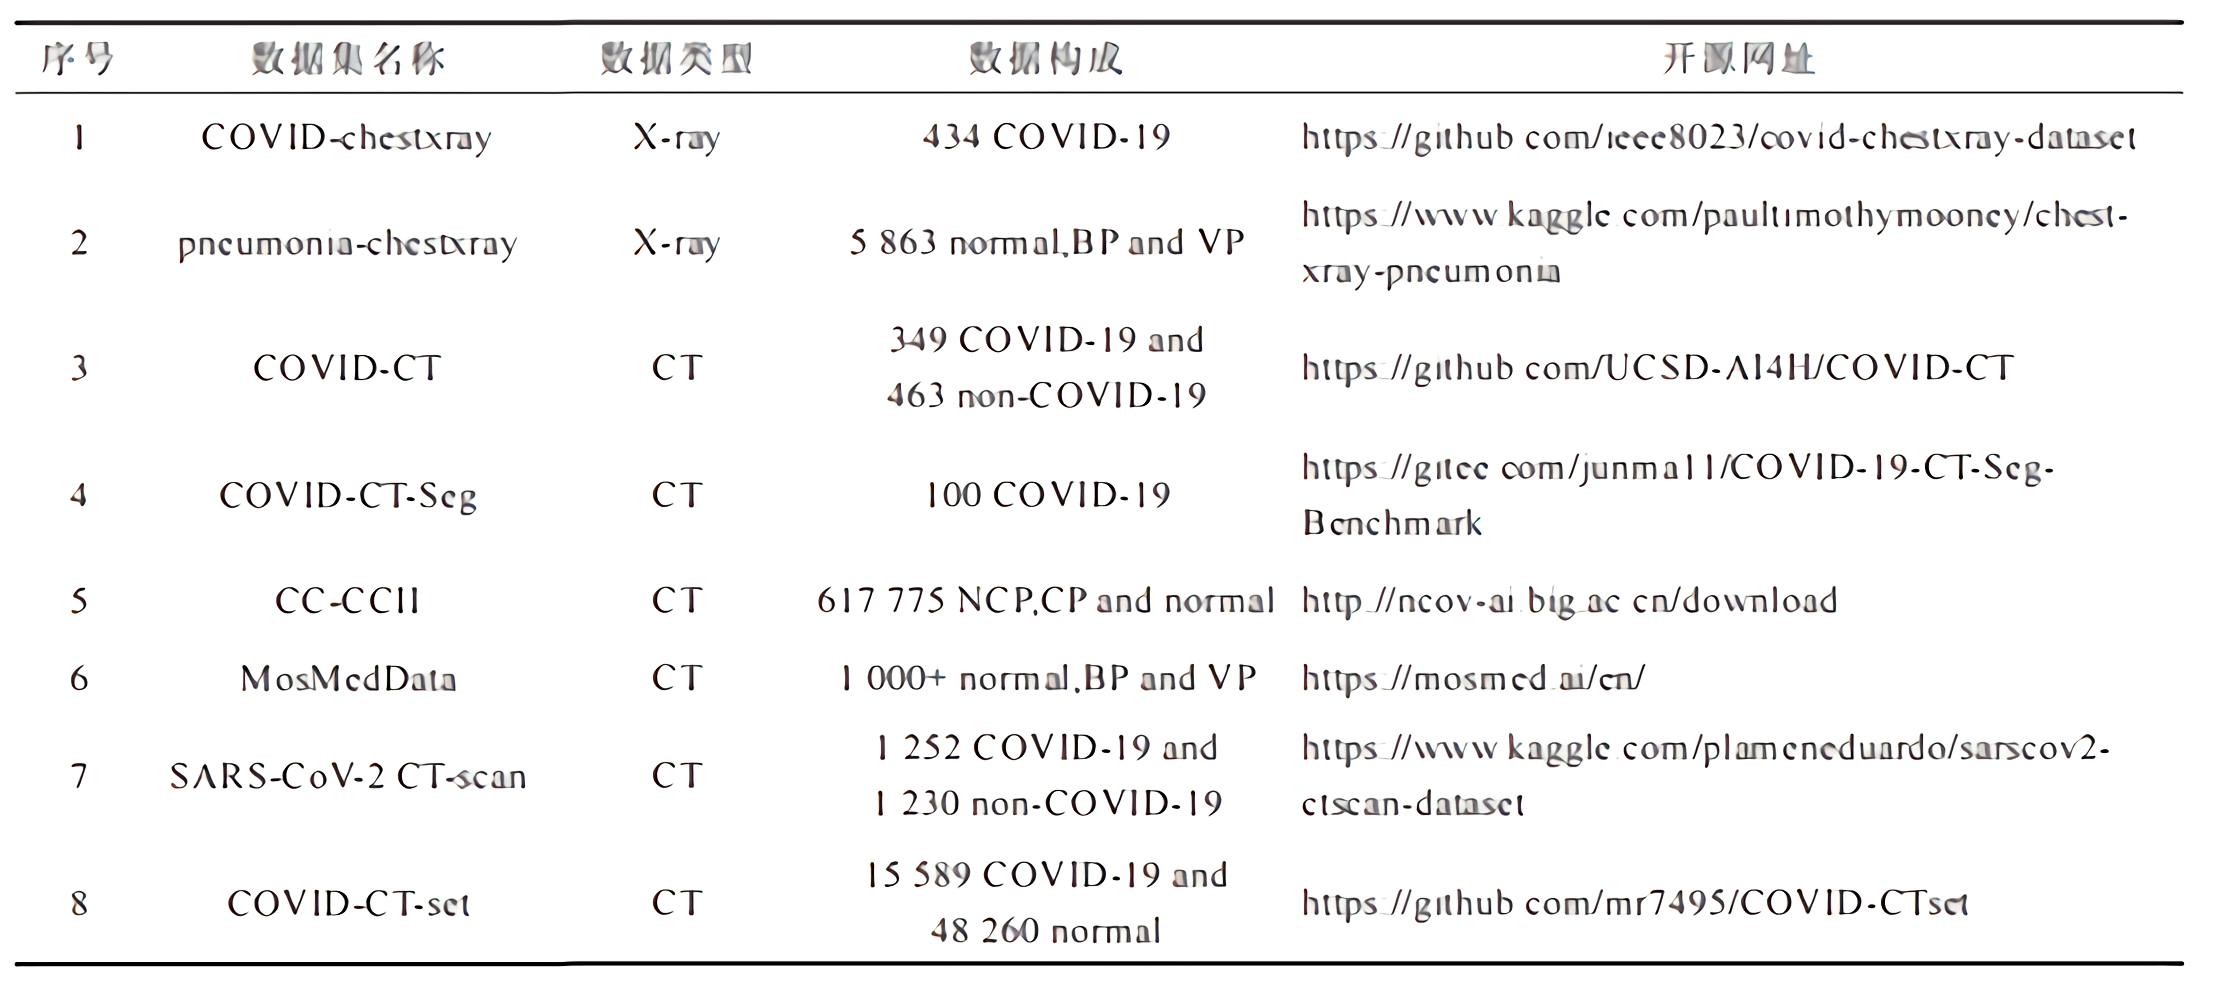
\includegraphics[width=0.5\textwidth]{img/fig0.png}
\caption{COVID-19相关的开源数据集}
\label{fig:COVID-19_dataset}
\end{figure}
\subsection{X-ray数据集}
常见的X-ray数据集主要包括COVID-chestxray和pneumonia-chestxray,下文进行具体介绍。
\subsubsection{COVID-chestxray数据集}
COVID-chestxray是一个公开的COVID-19病例数据集,包含COVID-19、其他病毒性肺炎和细菌性肺炎(MERS、SARS、ARDS)患者的胸部X-ray和CT图像,图像主要来自在线开源数据、网站和文献中所提到参考文献。此外,数据集作者允许用户通过github网站向该数据集提交其他COVID-19数据。该数据集主要包含434张COVID-19的X-ray正面视图,只有少量的CT图像。
\subsubsection{pneumonia-chestxray数据集}
pneumonia-chestxray数据集由训练集、测试集和验证集组成,包含健康受试者、非COVID-19病毒性肺炎患者和细菌性患者的5863张X-ray图像。其中,前后胸部X-ray图像选自广州市妇幼保健中心的1岁 $ \sim $ 5岁儿童患者的回顾性研究。数据集作者对所有数据进行了筛查,通过去除所有低质量或不可读的扫描图来进行质量控制。然后,由两名专业医师对图像进行诊断并给出对应的标签。此外,为尽可能减少人为标记带来的误差,由第三位专家对前两位医师的标记结果进行检查。值得注意的是,pneumonia-chestxray是非COVID-19数据集,但是大量研究者构建的COVID-19数据集部分采用该数据集中的健康受试者、病毒性肺炎患者和细菌性肺炎患者的X-ray数据进行增强。
\subsection{CT数据集}
常见的CT数据集主要包括COVID-CT、COVID-CT-Seg、CC-CCII、MosMedData、SARS-CoV-2CT-scan和COVID-CT-set,下文进行具体介绍。
\subsubsection{COVID-CT数据集}
COVID-CT数据集包含216名COVID-19患者的349张CT切片和非COVID-19患者的463张CT切片。该数据集主要收集来自网站和出版物的医学影像,即从760份COVID-19相关预印本文献中收集,这些文献主要来自medRxiv和bioRxiv。此外,对于每个CT图像,数据集作者还收集了从论文中提取的meta信息,如患者年龄、性别、位置、病史、扫描时间、COVID-19的严重程度和放射学报告。该数据集有两个主要缺点:首先,许多CT图像中含有CT扫描机或医生产生的标记,这可能对深度学习技术产生负面影响;其次,每个病人只有少数几张CT图像而不是一个完整的3D扫描体,无法使用3DCNN来挖掘肺部深层次信息。
\subsubsection{COVID-CT-Seg数据集}
COVID -CT-Seg 数据集是一个公开可用的 CT 数  据集 。数据集作者对来自意大利医学和介入放射学  学会网站上的 JPG 数据进行处理,其中包含 40 多个  COVID - 19 患者的 100 张轴向 CT 图像 。这些经由放  射学专家分割的图像包含毛玻璃、硬化和胸腔积液  三类标签 。该数据集于 2020 年 4 月 20 日进行更新, 增加 了 20 个标记 良好 的扫描样本数据,包括左肺、 右肺和病变感染区域的标记 。新增数据的注释工作  由三位经验丰富的放射科医生全程参与,其中两位放射科医生进行标记,一位进行验证。
\subsubsection{CC-CCII数据集}
CC-CCII 数据集是一个可公开使用 的 CT 数据 集,是目前针对 COVID- 19建立的最大CT数据集之一, 包含4 154名患者的6752次扫描结果,共计617775张CT  切 片 ,包 括 新 型 冠 状 病 毒 性 肺 炎(Novel  Corona  Pneumonia,NCP)、普通肺炎(Common Pneumonia,CP)和 正常对照组(normal)三大类 。其 中,肺炎包括细菌 性肺炎和病毒性肺炎 。然而,该数据集(2020 年 4 月 23 日发布的 1.0 版)包含了一些错误,如某些扫描中 存在 CT 图像次序混乱、部分扫描结果包含无用的头 部信息但不包括关键肺部信息等 。数据集作者于 2020 年7 月3 号发布 v2.2 版本,解决了压缩文件损坏 问题,同时增加了对应的病变分割数据集。
\subsubsection{MosMedData 数据集}
MosMedData 数据集包含 1 000 多位匿名患者的  胸部 CT 扫描数据 。数据集作者从 2020 年 3 月 1 日  至 4 月 25 日在莫斯科通过统一放射信息服务(URIS) 收集 。此外,数据集中的所有 CT 数据均带有特殊标  记 ,其根据分类进行标记 以反 映胸部 CT 肺组织 中  COVID - 19 的病理异常表现 。数据集根据标记将 CT  数据分为五大类,即从 CT-0(正常和无病毒性肺炎的  CT)到 CT-4(弥 漫性玻璃膜混浊 ,肺实质受 累超过
75\%)。 同时,为了更好地开发 AI算法,CT 薄切片被 转换为 NIFTI 格式 。在相应 的标记 中,病例 的整体 标记用于患者的自动分类,定位标记用于为放射科 医生指出在 CT 扫描中可疑的位置,病理轮廓标记用 于肺部病变的自动定量评估和患者两次 CT 之间的 动态评估 。此外,专家 明确标记 了其 中 50 个 CT 扫 描集 ,每个 CT 切 片 上 都标 出 了 COVID - 19 特 有 的 毛 玻 璃 混 浊 和 硬 化 的 像 素 区 域 ,并 显 示 出 肺 组 织 异常。
\subsubsection{SARS-CoV-2 CT-scan 数据集}
SARS-CoV-2 CT-scan 是一个公共可用的 SARS-  CoV-2 CT scan 数据集,包含 1 252 例 SARS-CoV-2感 染 阳性( COVID - 19)的 CT 扫描数据和 1 230 例未感 染 SARS-CoV-2 的患者 的 CT 扫描数据 。这些数据 是从巴西圣保罗的医院的真实患者处收集的 。该数 据集发布的目的是鼓励研究和开发人工智能算法, 旨在通过该数据集中的 CT 扫描数据进行训练测试
分析,确定病人是否被 SARS-CoV-2感染。
\subsubsection{COVID-CT-set数据集}
COVID -CT-set 数 据 集 包 含 95 例 COVID - 19 患 者 的 15 589 张 CT 扫描 图像和 282 例正常受试者 的 48 260 张 CT 扫描 图像 ,收集 于伊 朗 的一家 医疗 中 心 。为了保护患者的隐私,数据集作者将数据格式 从 DICOM 转换为 TIFF 。该数据集采用 16 位灰度数 据,能够避免 8位数据引起的信息丢失问题 。此外,将图像的每个像素值除以其最大像素值,从而得到 32 位浮点类型的像素值,使得图像能够在常规的监 视器中显示。

在 X -ray 数据集方面,pneumonia-chestxray 包含 大量非 COVID - 19 肺炎数据 ,该数据集被广泛用 于 基于深度学习的其他肺炎检测诊断模型,是一个成 熟且丰富的公共数据集,COVID -chestxray 则由于包 含 COVID - 19 样本而被大多数研究人员所熟知 。上 述两个数据集通常以组合的形式,共同参与基于深 度学习的 COVID - 19诊断模型的数据集构建 。而 CT  数据集相对 X -ray 数据集拥有更多 的 COVID - 19 样 本 数 据 ,甚 至 包 含 大 量 专 家 给 出 的 标 记( 如 MosMedData 数据集),能够更好地训练基于深度学习 的 COVID - 19检测诊断模型 。但是,上述 CT 公开数 据集提出时间较短,还未得到科研人员的广泛使用, 更多的科研工作者使用私有数据集进行模型的训 练 。综上,数据集在数量和质量方面还有待进一步 提高 ,使得科研人员构建 的 COVID - 19 检测诊断模 型能够在一个公平完善的基础上进行比较。
\section{评价指标}
基于深度学习的新冠肺炎诊断属于典型的医学图像处理问题,可以划分为分类任务和分割任务。对于分类任务,深度学习神经网络需要正确识别医学影像数据中的COVID-19和non-COVID-19,其中non-COVID-19可以进一步细分为病毒型肺炎、细菌型肺炎和正常等,根据分类的种类数量,新冠肺炎诊断可以是二分类问题,也可以是多分类问题。对分割任务,深度学习神经网络需要在对整个肺部进行分割预处理的基础上,进一步对肺部的病灶区域进行分割,从而获得医生最关注的区域,最终根据感染区域的特征和大小完成医学影像数据中新冠肺炎的诊断。下文分别对分类和分割任务中不同的评价指标进行介绍。
\subsection{分类任务的评价指标}
分类任务涉及7种常用的评价指标,即表示敏感性的召回率(Recall)、精准率(Precision)、特异性(Specificity)、准确率(Accuracy)、F1-score、ROC(Receiver Operating Characteristic)曲线和AUC(Area Under Curve)指标。召回率、精准率和特异性指标分别如下所示:
%行间公式
\begin{equation}
\begin{array}{l}
R_{\text {Recall }}=\frac{N_{\mathrm{TP}}}{N_{\mathrm{TP}}+N_{\mathrm{FN}}} \\
P_{\text {Precision }}=\frac{N_{\mathrm{TP}}}{N_{\mathrm{TP}}+N_{\mathrm{FP}}} \\
S_{\mathrm{Specificity}}=\frac{N_{\mathrm{TN}}}{N_{\mathrm{TN}}+N_{\mathrm{FP}}}
\end{array}
\end{equation}

其中,NTP表示实例为阳性并且被预测为阳性所对应的数量,NFN表示实例为阳性但被预测为阴性所对应的数量,NFP表示实例为阴性但被预测为阳性所对应的数量,NTN表示实例为阴性并且被预测为阴性所对应的数量。由于召回率和精准率被作为单一指标进行评估,因此无法全面地评估诊断结果。同时,针对不同场景的分类应用,对召回率和精准率的要求也有所不同。因此,出现了F1-score。该指标综合考虑了以上两个指标,可以表示为两者的调和平均,如式(2)所示:
%行间公式
\begin{equation}
\begin{array}{l}
F_{\text {1-score }}=\frac{2\times R_{\text {Recall }} \cdot P_{\text {Precision }}}{R_{\text {Recall }}+P_{\text {Precision }}}
\end{array}
\end{equation}

在更一般的情况下,该指标对应的形式如式(3)所示,其中,$\beta$为加权系数,用于调节召回率和精准率之间的权重关系。
%行间公式
\begin{equation}
\begin{array}{l}
F_{\beta}=\frac{\left(1+\beta^{2}\right) \cdot P_{\text {Precision }} \cdot R_{\text {Recall }}}{\beta^{2} \cdot P_{\text {Precision }}+R_{\text {Recall }}}
\end{array}
\end{equation}

F0.5-score和F2-score在统计学中均有广泛应用。新冠肺炎具有严重的危害性,在COVID-19诊断中必须保证足够高的敏感性,因此,推荐使用F2-score。准确率表达式如下:
%行间公式
\begin{equation}
\begin{array}{l}
A_{\text {Accuracy }}=\frac{1}{N}\left(N_{\mathrm{TP}}+N_{\mathrm{TN}}\right)
\end{array}
\end{equation}

其中,N表示样本实例的总数量。ROC曲线的横轴是伪阳性率(FalsePostiveRate,FPR),满足FPR=1-SSpecificity,纵轴是真阳性率(TruePostiveRate,TPR),满足TPR=RRecall。具体地,给定一个阈值,对所有实例进行分类预测,从而计算得出对应的一组(FPR,TPR)。最理想的情况为TPR=1,FPR=0。因此,ROC曲线越靠近坐标(0,1),说明算法性能越优秀。此外,ROC曲线具备一个很好的特性,即当测试集中的正负样本分布发生变化时,ROC曲线能够保持不变。通常实际数据集中存在类不平衡现象,即正、负样本数量差异较大。因此,ROC曲线得到了广泛的应用。AUC表示ROC曲线下的面积,用以评估分类器的优劣,对应的数值越大,代表算法性能越好。
\subsection{分割任务的评价指标}
分割任务涉及5种常用的评估指标,包括DICE系数、体积重叠误差(Volumetric Overlap Error,VOE)、相对体积差(Relative Volume Difference,RVD)、对称位置的平均表面距离(Average Symmetric Surface Distance,ASD)和对称位置的最大表面距离(Maximum Symmetric Surface Distance,MSD)。首先定义标识符Vgt和Vseg,以Vgt表示ground truth对应的分割结果,以Vseg表示预测的分割结果。

DICE系数作为分割任务中最常用的评价指标被广泛使用,其表达式如下:
%行间公式
\begin{equation}
\begin{array}{l}
    D_{\text {DICE }}=\frac{2 \cdot\left(V_{\text {seg }} \cap V_{\mathrm{gt}}\right)}{V_{\text {seg }}+V_{\mathrm{gt}}}
\end{array}
\end{equation}

DICE系数类似,VOE将交集运算替换为差集运算表示错误率,其表达式如下:
%行间公式
\begin{equation}
\begin{array}{l}
V_{\mathrm{VOE}}=\frac{2 \cdot\left(V_{\mathrm{seg}}-V_{\mathrm{gt}}\right)}{V_{\mathrm{seg}}+V_{\mathrm{gt}}}
\end{array}
\end{equation}

RVD表示Vgt和Vseg两者体积间差异,其表达式如下:
%行间公式
\begin{equation}
\begin{array}{l}
R_{\mathrm{RVD}}=\left(\frac{V_{\mathrm{seg}}}{V_{\mathrm{gt}}}-1\right) \times 100 \%
\end{array}
\end{equation}

为计算ASD,先定义Aseg表示预测的分割结果Vseg中的边界像素,Agt表示groundtruth中的边界像素。由此计算Bseg:
\begin{equation}
\begin{array}{l}
B_{\text {seg }}=\left\{\forall p_{1} \in A_{\text {seg }}, d\left(p_{1}, p_{2}\right) \mid \exists p_{2} \in A_{\mathrm{g}}\right\}
\end{array}
\end{equation}

其中,d表示边界像素之间的最短距离。同理可计算得到Bgt。根据计算得到的Bseg和Bgt,对应ASD的表达式如下:
\begin{equation}
\begin{array}{l}
A_{\mathrm{ASD}}=\min \left(\left\{B_{\mathrm{seg}}, B_{\mathrm{gt}}\right\}\right)
\end{array}
\end{equation}

MSD则与ASD的定义类似,将其中的平均运算替换为最大值运算,其表达式如下:
\begin{equation}
\begin{array}{l}
M_{\mathrm{MSD}}=\min \left(\left\{B_{\mathrm{seg}}, B_{\mathrm{gt}}\right\}\right)
\end{array}
\end{equation}
\section{深度学习在COVID-19检测模型中的可优化步骤}
\subsection{图像的特征提取与融合}
在图像分类研究中,为了减少分类器需要学习的像素数量,可以进行特征提取。从医学图像中可以提取的特征包括影像组学特征和深度特征。

影像组学提取传统的图像特征,包括形态特征(表面体积比、致密度、偏心度、球形度等)、一阶直方图特征(描述与ROI内的体素强度分布有关的特征均数、中位数、最小值、最大值、标准差、偏度和峰度等)和二阶直方图特征。二阶直方图特征是图像的纹理特征, 研究中常采取Haralick等人提出灰度共生矩阵法(GLCM, Gray-level co-occurrence matrix)和由Ojala等人提出的局部二值模式(LBP,Local Binary Pattern)。

在医学图像研究中,常常利用CNN(卷积神经网络),GCN(图卷积神经网络)、U-Net等结构来提取深度特征。CNN已被广泛用于图像分析。CNN都由三种类型的层组成,包括卷积层、池层和全连接层。其中,第一层卷积层用于提取边缘等低级图像特征,后续的卷积层提取图像的高级特征。对于图像特征提取问题,由于医学图像往往数据量小,且是多模态的,基于结构较为简单的U-Net结构便于设计网络提取特征。

在特征提取过程中,迁移学习被广泛使用。通常,从头开始训练一个深度 CNN 需要很长时间,而训练后的 CNN 的表现可能远不能令人满意。而迁移学习可以节省训练时间,并取得更好的训练效果。在迁移学习中,把在不同数据集上训练好的网络作为基础网络,利用待研究的数据集可以训练调整后的网络。该网络常常用作特征提取器,为分类器提供提取的特征。Xiang Yu等人加载了在 ImageNet 上预先训练的 CNNs,从其中的一个大小为1000的全连接层中提取特征。

对于不同的特征,研究中利用多模态融合策略来集成,消除不同模态的异质性差异, 联合架构是将多模态空间映射到共享语义子空间中,从而融合多个模态特征,而传统的特征融合算法主要可以分为三类:基于贝叶斯决策理论的算法、基于稀疏表示理论的算法、基于深度学习理论算法。

多模态联合架构的关键是实现特征“联合”,一种较简单的方法是直接连接,即“加”联合方法。该方法在不同的隐藏层实现共享语义子空间,将转换后的各个单模态特征向量语义组合在一起,从而实现多模态融合,如式(11)所示:
%行间公式
\begin{equation}
    z=f\left(w_{1}^{T} v_{1}+w_{2}^{T} v_{2}+w_{3}^{T} v_{3}+\cdots+w_{n}^{T} v_{n}\right)
\end{equation}
其中,z 是共享语义子空间中的输出结果,v 是各单模态的输入,w 是权重,下标表示不同的模态,通过映射 f 将所有子模态语义转换到共享子空间。

在Wang等人的研究中,他们设计了一个融合CT图像和临床数据的DCNN模型,以充分利用两种不同类型的数据,实验过程如图2所示:
%插入图片
\begin{figure}
\centering
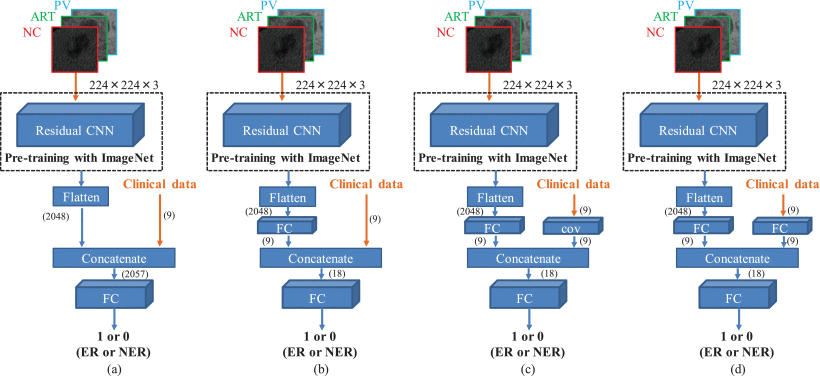
\includegraphics[width=0.5\textwidth]{img/fig4.png}
\caption{CT图像和临床数据的DCNN模型}
\label{fig:CT_DCNN}
\end{figure}

他们做了一个对比实验,其区别之处在于(a)实验将Flatten后的2048个影像特征直接与9个Clinical data连接,而(b)组实验,则将2048个影像特征经过一个FC层(全连接层)的处理,处理为9个特征再与9个Clinical data连接,而(c)实验则是在(b)实验的基础上,将Clinical data经过一个COV层的处理,(d)实验则是在(b)实验的基础上,将Clinical data经过一个FC层的处理。其实验结果如图:
%插入图片
\begin{figure}[h]
\centering
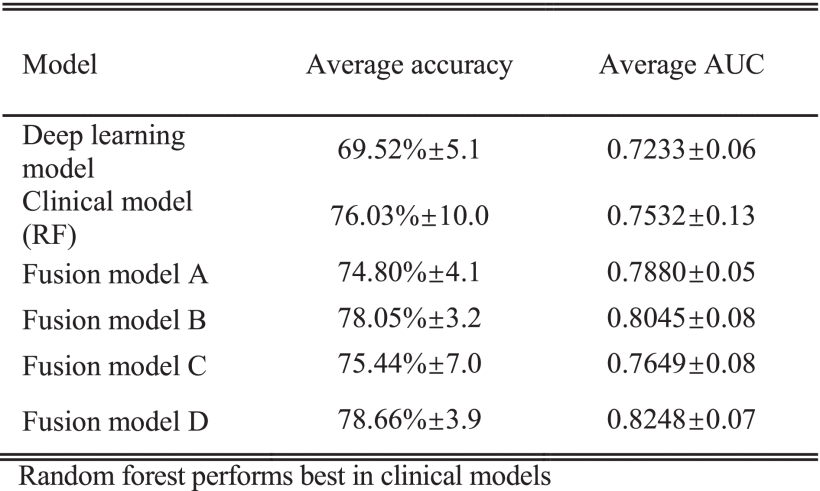
\includegraphics[width=0.5\textwidth]{img/fig5.png}
\caption{对比实验结果图}
\label{fig:result}
\end{figure}

从结果中可以预见的是,经过处理的融合结果会优于简单暴力的直接缝合。

而除了简单的线性拼接之外,在输入特征水平上的多模态还有很多种方法,诸如TFN(Multimodal Tensor Fusion Network)、LMF(Low-rank Multimodal Fusion),这类深度学习优化方法在新冠肺炎辅助诊断的运用中尚不成熟,具有很大的发展空间。

下面将简单的介绍上述的几种方法:
\subsubsection{TFN(Multimodal Tensor Fusion Network)}
首先是基于矩阵的TFN,TFN属于early fusion,是一个典型通过矩阵运算进行融合特征融合的多模态网络,即直接对三种模态的数据(如Text,Image,Audio)的三个特征向量X,Y,Z,进行:
%行间公式
\begin{equation}
h_{m}=\left[\begin{array}{c}
h_{x} \\
1
\end{array}\right] \otimes\left[\begin{array}{c}
h_{y} \\
1
\end{array}\right] \otimes\left[\begin{array}{c}
h_{z} \\
1
\end{array}\right]
\end{equation}
便得到了融合后的结果m,如图4所示。
%插入图片
\begin{figure}[h]
\centering
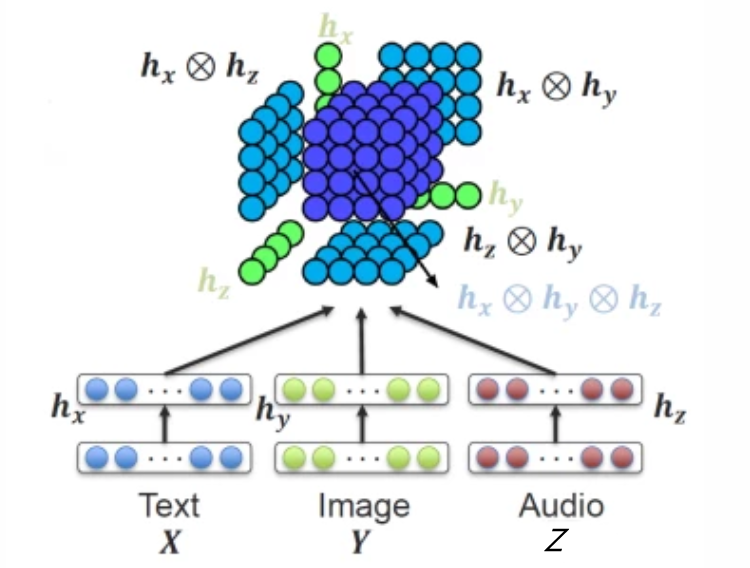
\includegraphics[width=0.5\textwidth]{img/fig6.png}
\caption{TFN网络结果图}
\label{fig:TFN}
\end{figure}
缺点:TFN通过模态之间的张量外积(Outer product)计算不同模态的元素之间的相关性,但会极大的增加特征向量的维度,造成模型过大,难以训练。
\subsubsection{LMF(Low-rank Multimodal Fusion)}
是TFN的等价升级版,就具体模型如图。LMF利用对权重进行低秩矩阵分解,将TFN先张量外积再FC的过程变为每个模态先单独线性变换之后再多维度点积,可以看作是多个低秩向量的结果的和,从而减少了模型中的参数数量。
%插入图片
\begin{figure}[h]
\centering
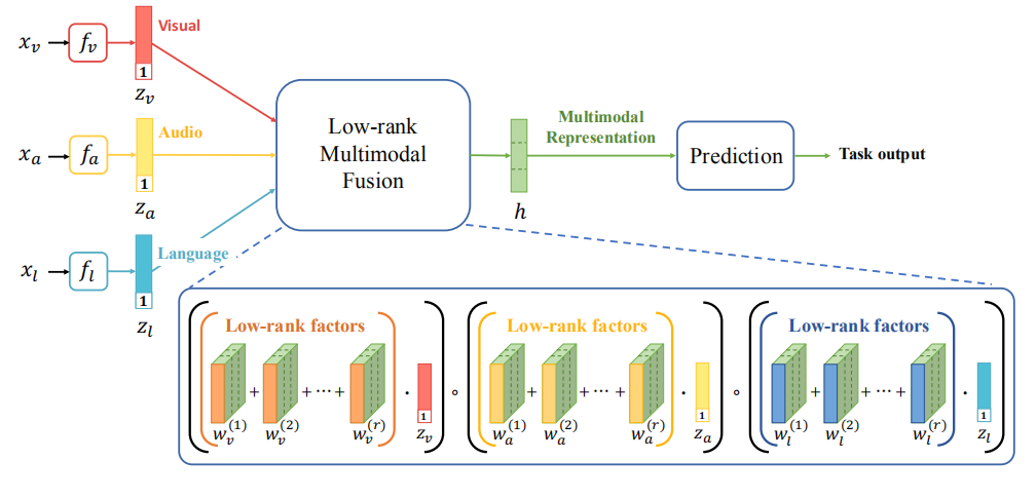
\includegraphics[width=0.5\textwidth]{img/fig7.png}
\caption{LMF网络结果图}
\label{fig:LMF}
\end{figure}
缺点:虽然是TFN的升级,但一旦特征过长,仍然容易参数爆炸。
\subsection{图像的分割与分类}
多数医疗影像分割任务都会首先用U-Net作为baseline。U-Net是2015年U-Net: Convolutional Networks for Biomedical Image Segmentation提出的模型,经过4次encoder(下采样)后进行4次decoder(上采样),将encoder得到的高级语义特征图恢复到原图片的分辨率。相比于FCN和Deeplab等结构,UNet在同一个阶段使用了skip connection(残差连接),而不是直接在高级语义特征上进行监督和误差反传,这样就保证了最后恢复出来的特征图融合了更多的浅层特征,使得不同规模的数据得到了的融合。由于医学影像数据集的限制, U-Net参数量更少,信息利用率高,不容易过拟合,因此U-Net及其变体网络(3D U-Net、U-Net++、Attention U-Net和transUnet等)被广泛应用于医学图像的分割。Zheng等人就用Unet网络进行肺部区域的分割。
%插入图片
\begin{figure}[h]
\centering
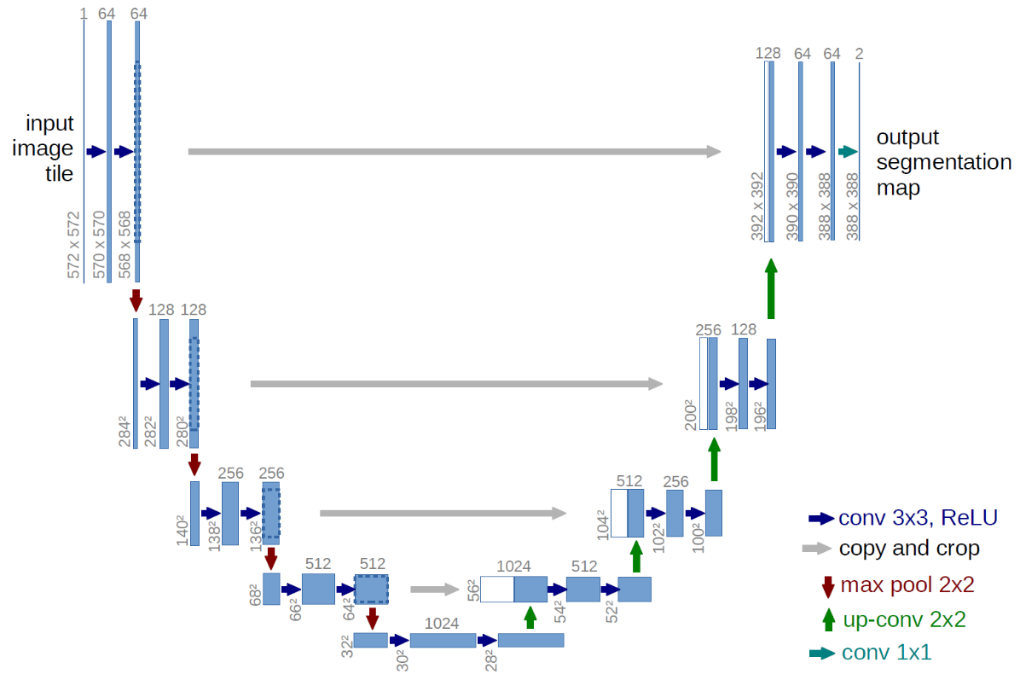
\includegraphics[width=0.5\textwidth]{img/fig8.png}
\caption{U-Net网络结构图}
\label{fig:U-Net}
\end{figure}

transUnet结构如图7所示,它利用了一个混合了CNN-Transformer结构作为编码器,并且用一个级联的上采样器保证精确预测。它与传统的Unet相比,增加了自注意力机制,因此更能完成长距离依赖建模。
%插入图片
\begin{figure}[h]
\centering
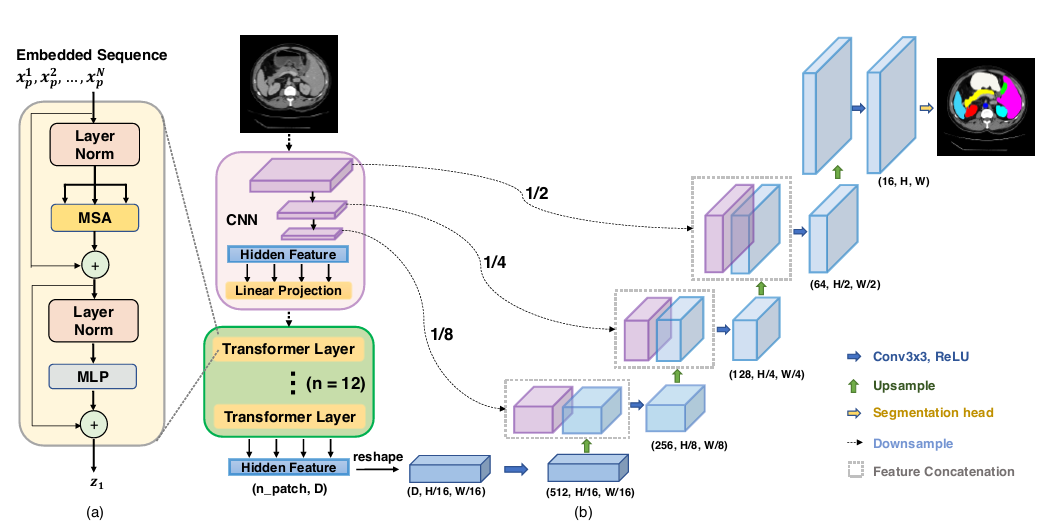
\includegraphics[width=0.5\textwidth]{img/fig9.png}
\caption{transUnet网络结构图}
\label{fig:transUnet}
\end{figure}

Attention Unet结构如图8所示,它通过添加Attention Gate,在保持计算效率的情况下,提高了分割模型的精度。Gaál等人(2020)采用生成对抗网络和Attention U-Net设计了肺部区域分割网络。
%插入图片
\begin{figure}[h]
\centering
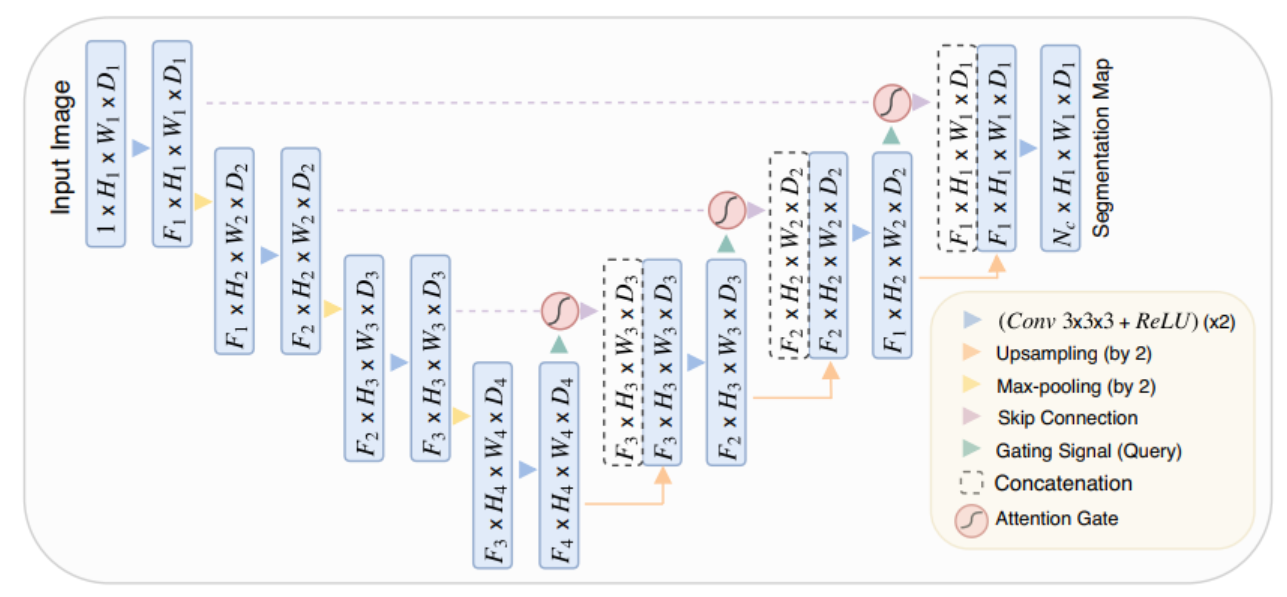
\includegraphics[width=0.5\textwidth]{img/fig10.png}
\caption{Attention U-Net网络结构图}
\label{fig:Attention U-Net}
\end{figure}

UNet在图像分割任务中具有大量的应用。目前虽然也有许多新的方法在此基础上进行改进,但几乎没有人对这些改进版本做过比较综合的比较。由于同一个网络结构可能在不同的数据集上表现出不一样的性能,在具体的任务场景中还是要结合数据集来选择合适的网络。研究中常用的基础分类模型主要可分为以下几种。
%插入图片
\begin{figure}[h]
\centering
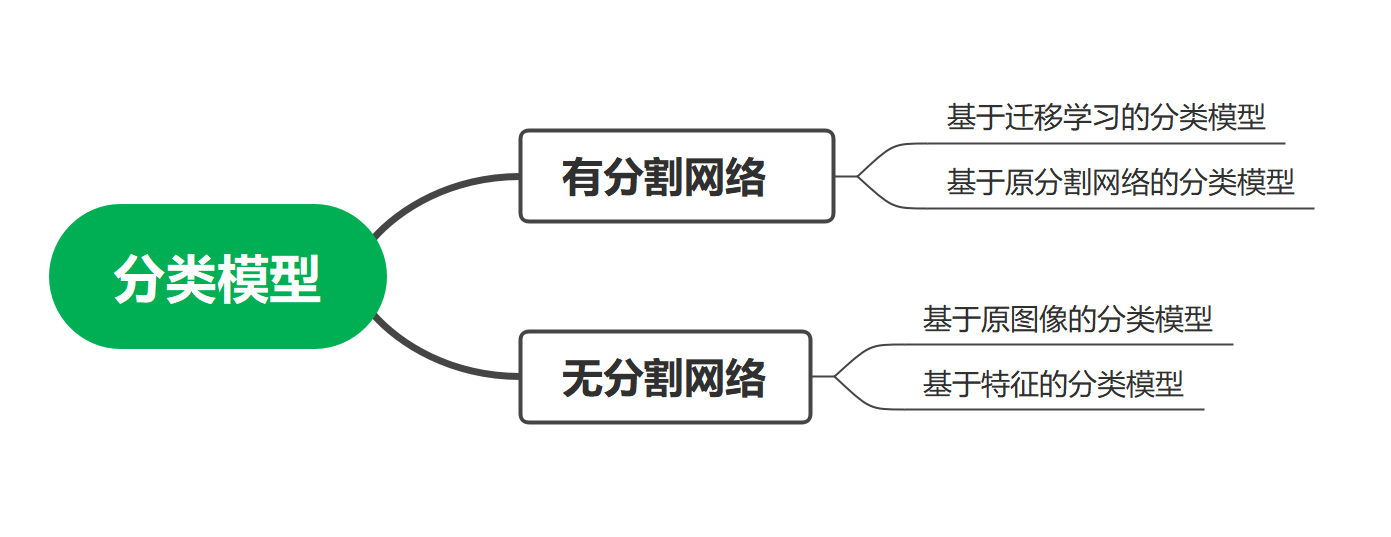
\includegraphics[width=0.5\textwidth]{img/fig11.png}
\caption{分类模型种类}
\label{fig:VGG-16}
\end{figure}

有分割网络模型的诊断系统一般由两部分组成:肺病灶分割模型与诊断分类模型。基于原分割网络的分类模型可以直接肺病变图作为分割网络生成的输入,并进行分类操作。虽然真实世界的原始扫描包含噪声并且因不同的设备和人类操作而异,但这种方法在临床实施过程中提供了更好的泛化和互操作性,相比于简单的端到端的黑盒网络而言表现出了更好的效果。 基于迁移学习的分类模型则通常将处理自然图像的分类网络(如AlexNet和VGG19)迁移用作处理医学图像上。目前应用到医学图像分类的迁移学习主要有微调法和特征提取法。在微调法(fine-tunning)中,迁移学习对训练过的网络的权重进行微调后,设置新的全连接层,并在特定分类任务中进行训练。在特征提取(feature extraction)中,将医学图像输入到已经在训练过的CNN之后,提取某一层的输出作为传统分类器(如支持向量机SVM)的输入特征(如图10)。
%插入图片
\begin{figure}[h]
\centering
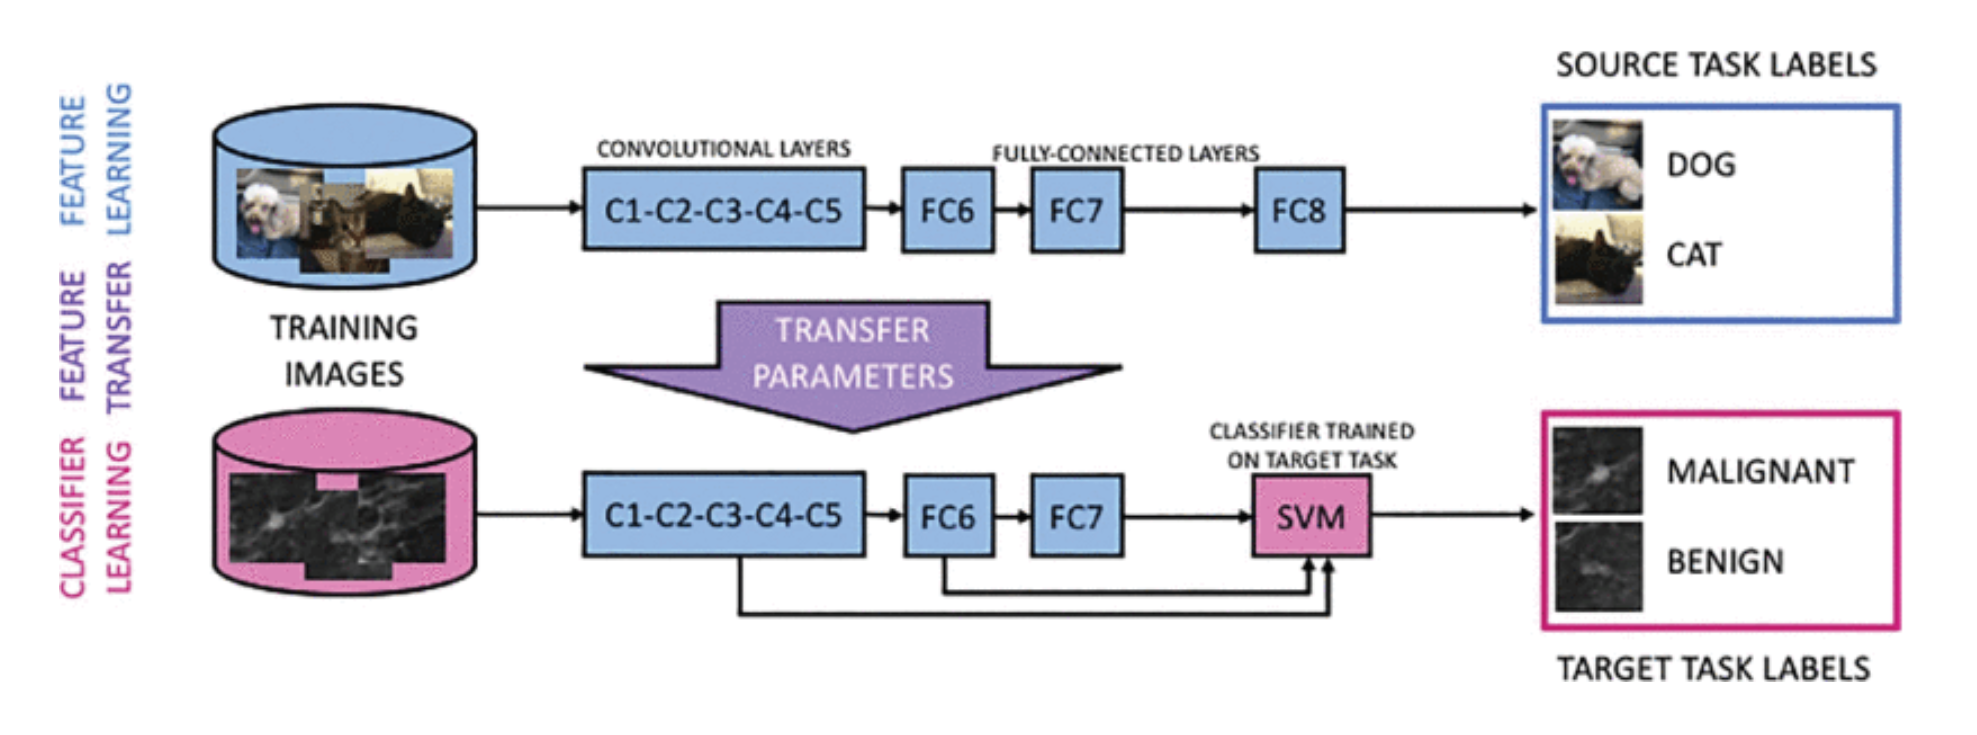
\includegraphics[width=0.5\textwidth]{img/fig12.png}
\caption{特征提取法}
\label{fig:feature extraction}
\end{figure}

对于没有分割网络的分类模型,第一种方法是事先提取出能与标签表现出相关关系的特征用于分类。例如,在这篇文章中,作者团队利用来自 GLCM的64个值、6个纹理运算符和来自本地二进制模式的59个值作为前馈神经网络的输入值。第二种方法是直接将预处理后的图像展平后输入深度学习网络中进行分类。例如在这篇文章中,作者应用了缩放共轭梯度反向传播训练的前馈神经网络和卷积神经网络进行分类。

目前,医学图像分类领域广泛使用卷积神经网络(Convolutional Neural Networks, CNN)构建深度学习模型。Hamidian 等提出两段检测网络,第一阶段使用三维FCN筛选疑似病灶区域,第二阶段使用三维CNN对被试进行分类。Gao等提出将二维CNN和三维CNN结合,根据得到的Softmax分数的平均值协调两个CNN网络分类。Silva等采用粒子群优化(PSO)算法对CNN中的网络超参数进行优化,提高了分类网络的性能。

上述分割或分类的方法只针对单一的任务,在获取特征时往往会忽略一些任务之间相关联的信息,不能得到更佳的分割或分类性能。为了更好地利用分割和分类任务之间的关联信息,提升分割和分类的精度,He等使用了多任务学习(Multi-Task Learning,MTL)模型,该模型的编码部分使用DenseNet/ResNet结构,解码部分使用上采样和级联操作,其呈现出非对称结构的端对端学习网络,在最后分为分割和分类两支输出,借助分类任务辅助学习关联信息提升分割精度。Y-Net采用了两阶段结构,其第一部分像U-Net一样输出分割掩模,第二部分在底层热图处添加输出分类标签的并行分支。
%插入图片
\begin{figure}[h]
\centering
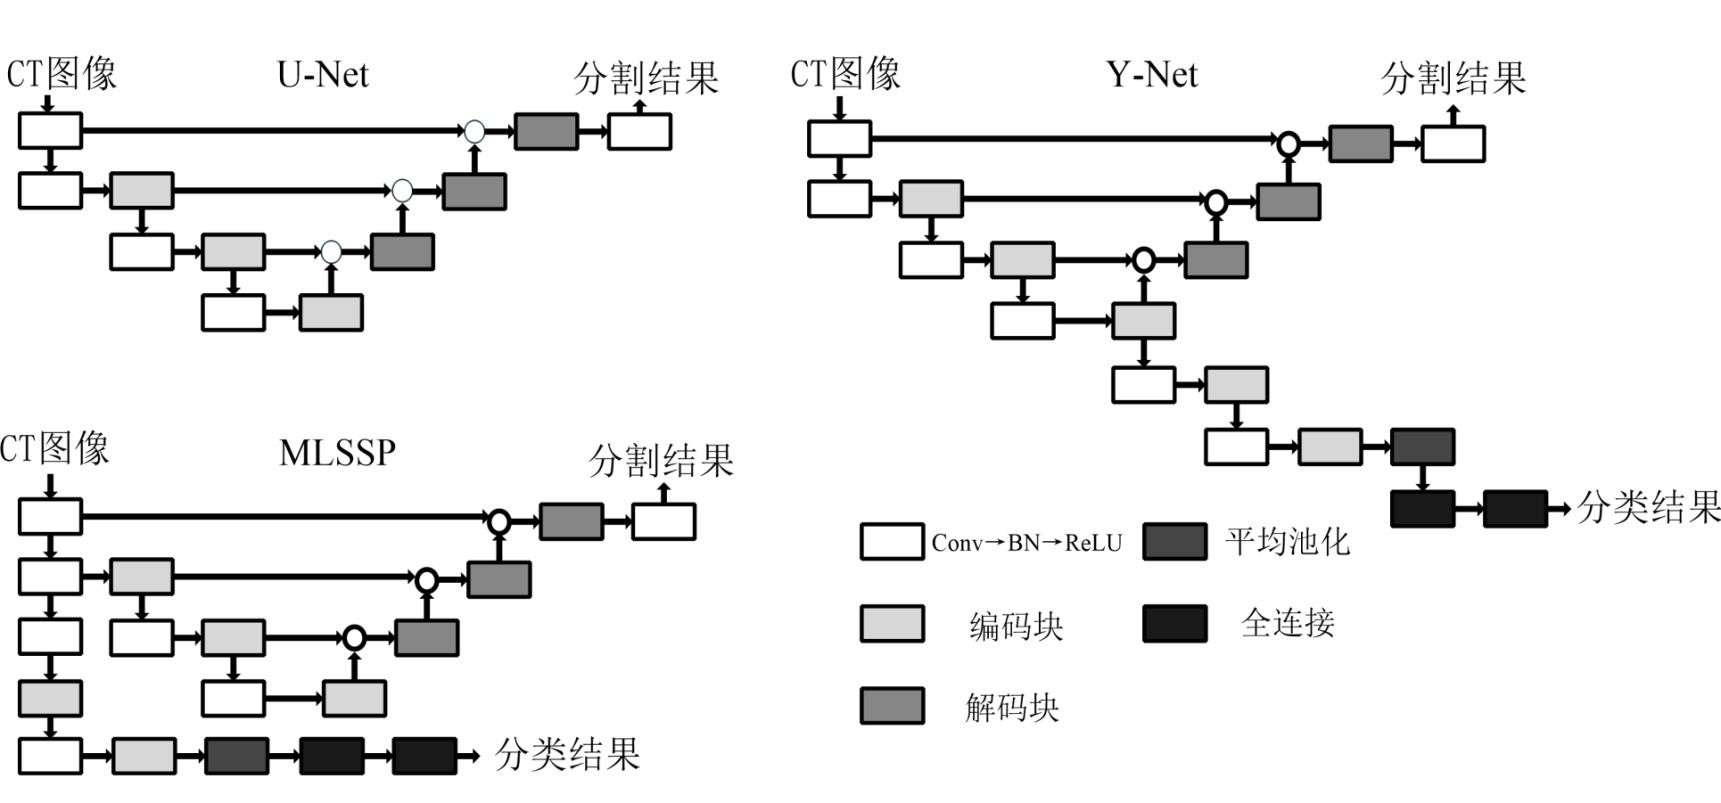
\includegraphics[width=0.5\textwidth]{img/fig13.jpg}
\caption{三种结构对比}
\label{fig:multi-task learning}
\end{figure}
\subsection{多任务学习与级联}

Liu等提出,与单独训练相比,联合训练级联网络可以提高模型的泛化能力和性能。本文将这种方法视为多任务学习,其中单个网络可以产生多个输出,相关的多任务网络结构设计通常涉及到任务相关提示、深度监督和中间信息等概念。这些概念的相同之处在于都额外添加了辅助的监督信号,而这种信号可以通过引入先验信息来规范和引导网络进行学习,从而提高模型的可解释能力。

现有的多任务学习方法通常都是基于U型网络结构直接进行扩展。Sun等提出将两个改进的U型网络(堆叠块)连接起来,用于在卫星成像上进行精确的道路分割,第一个块提供辅助信息,第二个块用来生成道路分割结果。Zhuang引入了LadderNet,它可以看作是一个由多个U型网络组成的链,与其他方法略微不同的是,其对特征的组合是通过求和的方式,而不是拼接。Murugesan等提出了Psi-Net,这是一种集成了1个编码器和3个并行解码器的网络结构,并用一个正则化损失对共享的编码器进行联合优化,同时使用2个解码器分别输出辅助信息,另外1个解码器输出分割图,提高了医学图像分割的准确性。

在设计多任务网路过程中,我们如何平衡不同类型的任务,避免在训练过程中,整个网络被简单任务主导,导致任务之间的性能差异巨大。这就涉及到为不同任务的loss function赋上不同的权重,将不同task之间的loss统一成一个损失函数,如果只是简单的将不同任务的loss相加,这样会造成最终模型在有些任务上表现很好,在有的任务上大失水准。背后的原因是不同任务的不同损失函数尺度有很大的差异,因此需要考虑用权值将每个损失函数的尺度统一,比如将不同的loss拉到统一尺度下,这样就容易统一,具体的办法就是利用同方差的不确定性,将不确定性作为噪声,进行训练。
%插入图片
\begin{figure}[h]
\centering
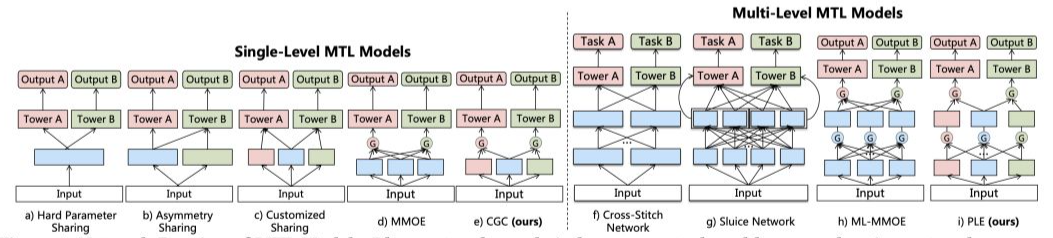
\includegraphics[width=0.5\textwidth]{img/fig14.png}
\caption{多任务学习}
\label{fig:multi-task learning}
\end{figure}

\section{基于深度学习的新冠肺炎辅助诊断模型}
我们小组打算从模型任务和影像数据类型,模型任务包括单任务(即分类任务或分割任务)和多任务(即分类任务和分割任务),对基于深度学习的COVID-19检测诊断模型进行分类与阐述。分类任务先对整个肺部区域进行提取,再使用卷积神经网络学习新冠肺炎的特征,从而实现对新冠肺炎的诊断;分割任务则在预处理(提取整个肺部区域)的基础上,进一步对肺部病灶区域进行了分割,能够更有效地对特征进行提取,从而改善新冠肺炎诊断的效果。但是,分割任务的实现依赖于额外的医学影像病灶标记,从现有数据集来看,相对于不带病灶标记的数据,带病灶标记的数据显得更加匮乏。基于深度学习的分类任务和分割任务处理流程分别如图13和图14所示,对两者进行组合即可得到多任务的处理流程。
%插入图片
\begin{figure}[h]
\centering
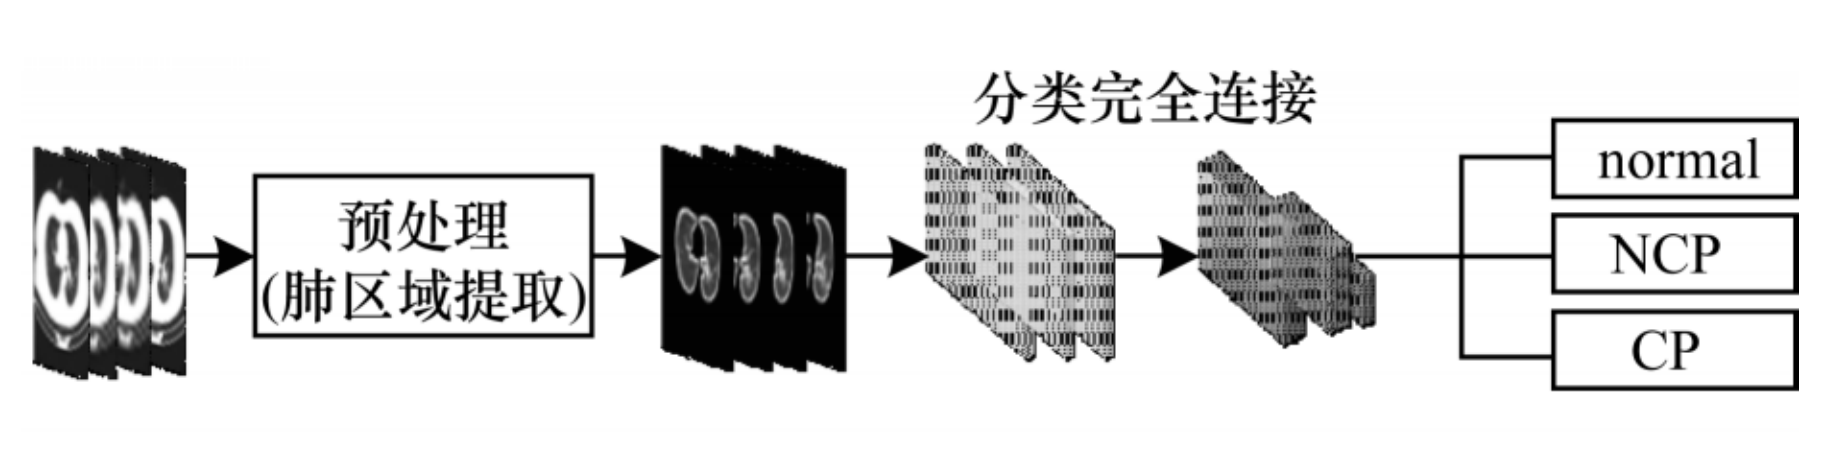
\includegraphics[width=0.5\textwidth]{img/fig2.png}
\caption{基于深度学习的分类任务处理流程}
\label{fig:COVID-19_classification_and_segmentation_process}
\end{figure}
%插入图片
\begin{figure}[h]
\centering
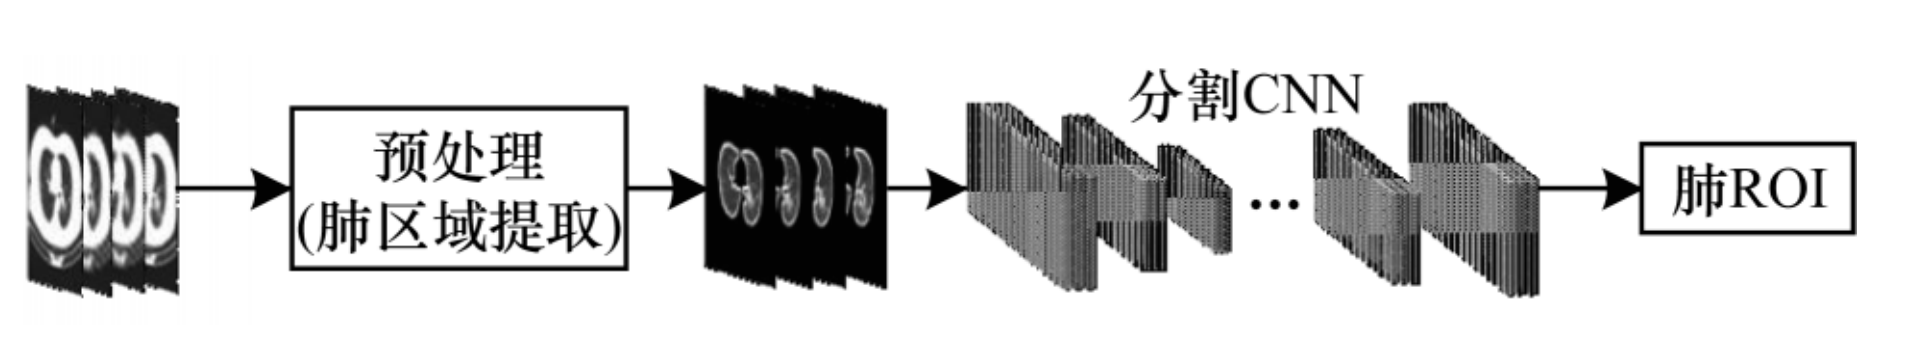
\includegraphics[width=0.5\textwidth]{img/fig3.png}
\caption{基于深度学习的分割任务处理流程}
\label{fig:COVID-19_classification_and_segmentation_process}
\end{figure}
\subsection{基于模型任务的分类}
\subsubsection{基于分割或分类任务的COVID-19诊断模型}

文献\cite{b1}设计了一种深度学习模型,从典型的病毒性肺炎中筛选COVID-19。首先,放射科医生将感染区域标注为感兴趣区域(RegionofInterest,ROI)。然后,作者构建基于Inception网络\cite{b2}的迁移学习神经网络用以提取特征向量,结合决策树和AdaBoost\cite{b3}对COVID-19和典型病毒性肺炎进行分类。该工作收集的数据集包括99例患者(44例COVID-19和55例典型病毒性肺炎)的胸部CT图像。该模型在内部测试数据集上的准确率为82.9\%,特异性为84\%,敏感性为81\%。

文献\cite{b4}使用ResNet50\cite{b5}提取特征,并添加特征金字塔网络(FeaturePyramidNetwork,FPN)\cite{b6}和注意力模块\cite{b7}构建诊断模型。首先,提取主要肺部区域,并用肺本身填充肺分割的空白,以避免因不同肺轮廓引起的噪声。然后,设计细节关系提取神经网络(DRE-Net)来提取CT图像中的细节区域,并进行图像级别的预测。最后,将图像级别的预测集合相结合以实现患者级别的诊断。该系统对88例COVID-19患者、101例细菌性肺炎患者和86例健康受试者的CT扫描数据进行了深度学习模型的训练和验证。在测试集中,模型的AUC为0.95,敏感性为96\%,其对肺炎分类(COVID-19或细菌性肺炎)的准确率为86.0\%,对肺炎诊断(COVID-19或健康)的准确率为94.0\%。

文献\cite{b8}使用了一个大型胸部CT数据集,包含3322名患者的4356张胸部CT图像(1296张COVID-19、1735张社区获得性肺炎(Community-AcquiredPneumonia,CAP)和1325张非肺炎)。具体地,该方法将ResNet50模型应用于具有共享权重的二维(2D)切片上,结合最大值池化(max-pooling)以区分COVID-19、CAP和非肺炎。实验结果表明,该模型可以准确检测COVID-19,并能有效区分社区获得性肺炎和其他肺部疾病。该模型的敏感性为90\%,特异性为96\%,AUC为0.96。

文献\cite{b9}使用UNet++\cite{b10} \cite{b11}提取COVID-19患者CT图像中的肺部病变区域,图像级别的标记(COVID-19或非COVID-19)直接根据分割的病变区域确定,而病例级别的标记则增加了一个连续图像预测结果的逻辑:将分割图像的预测结果分为四等份,只有当三张连续图像的病变分割出现在同一象限时,才判定病例为阳性。获得的数据集包括106例患者(51例为COVID-19,55例为其他疾病)的二维CT图像,且被随机分为训练集和验证集。该模型对COVID-19病例级别的检测诊断准确率达到95.2\%,敏感性达到100\%,特异性达到93.6\%。目前该模型已被部署到武汉大学人民医院以帮助放射科医生进行新病例的分析,并在互联网上开源,以实现对CT图像的快速审查。此外,此项研究使用了包括27名潜在患者数据的前瞻性数据集做进一步验证,表明模型取得了与专业放射科医生相当的性能,可使放射科医生的阅读时间减少65\%。

文献\cite{b12}提出一种基于DenseNet201的深度迁徙学习方法检测COVID-19,以判断患者是否被感染。该模型利用其在ImageNet数据集上学习的权值和卷积神经结构来提取CT图像中的特征。该文作者通过实验比较VGG16、InceptionResNet、ResNet152v2和DenseNet201等模型的性能表现。实验结果表明,DenseNet201模型的F1-score和准确率均为最佳。

\subsubsection{基于分割和分类任务的COVID-19诊断模型}

文献\cite{b13}使用ResNet18\cite{b14}自动检测CT图像中的感染区域,并使用ResNet23来识别感染区域是否为COVID-19症状。首先,利用ResNet18的分割模型从肺部CT图像中分割出候选感染区域。然后,利用ResNet23分类模型将候选区域分类到COVID-19、甲型流感病毒性肺炎或健康组,同时通过附带位置-注意力模型得到对应的置信分数。最后,利用噪声函数或贝叶斯函数计算感染类型和总置信度。CT样本数据集包括219例COVID-19患者、224例甲型流感病毒性肺炎和175例健康CT样本,该文作者随机抽取85.4\%的CT样本作为训练集,其余14.6\%的CT样本用于测试。在测试集上,该模型的敏感性达到了86.7\%,相对不使用位置-注意力模型提高了3.4\%。

文献\cite{b15}构造了一种用于筛选COVID-19患者的模型,该模型接收胸部CT图像,输出肺部异常定位和定量测量结果。模型主要由AB两个子系统构成。子系统A使用现成的商业软件对带有结节和病灶混浊的病例进行三维(3D)分析,子系统B对病例的切片进行二维分析,并使用U-Net分割网络提取感兴趣区域,且由2DResNet50模型\cite{b16}检测出COVID-19相关异常结果,最终实现较大弥漫性混浊的定位和病例的诊断。模型根据阳性率(阳性检出切片与肺切片的百分比)确定病例分类。研究结果表明,该模型在以阳性率1.9\%作为阈值的情况下,AUC为0.996,敏感性为96.4\%,特异性为98\%。

文献\cite{b17}收集了来自5家医院的1136例患者(723例COVID-19阳性、413例COVID-19阴性)的胸部CT图像。该文提出的诊断模型包含基于UNet++的分割模型和基于ResNet50的分类模型。分割模型用于突出肺部区域所有病变,以便快速检查,同时作为分类模型的输入。该模型的敏感性和特异性分别为97.4\%和92.2\%,满足临床应用需求。

文献\cite{b18}提出一种多任务学习(Multi-Task Learning,MTL)模型检测COVID-19,并对胸部CT图像中的病变区域进行分割。MTL将来自不同任务的若干信息进行组合,以提高模型的性能,使其具有更强的泛化能力。该模型由一个编码器和两个解码器组成,用于图像的重建和分割,同时包含一个用于分类的多层感知器(Multi-Layer Perceptron,MLP)。该文利用1044例患者的数据集(包括449例COVID-19患者、100例正常患者、98例肺癌患者和397例不同病理类型的患者)对所提出的模型进行评估,并对比其他图像分割和分类技术。该模型准确率为0.86,敏感性为0.94,特异性为0.79。

文献\cite{b19}采用多任务学习模型,提出一种卷积神经网络模型实现COVID-19检测和患者严重程度的细化。该文训练ResNet50作为分类网络,该网络以轴向切片作为输入,独立提取切片的特征向量,预测肺实质受累的概率,实现对COVID-19的有效检测,而患者严重程度量化任务的实现由两部分组成:左/右肺的分割和病变的分割。肺部的整体分割由一个标准的完全卷积神经网络完成,使用K-means算法对肺部内体素进行聚类,以欧几里得距离作为体素间的度量,完成左/右肺的分割。病变区域的分割则使用基于U-Net结构的网络完成。最后对两个体积的比率进行分级,依次对应不同的严重程度。该模型在COVID-19识别任务上AUC为0.951,在严重程度定量任务上,斯皮尔曼相关性系数达到0.98。
\subsection{基于影像数据类型的分类}
鉴于普通肺炎特别是病毒性肺炎与COVID-19有相似的影像学表现,其鉴别诊断将更有助于临床筛选过程。因此,基于深度学习的COVID-19诊断任务可以概括为健康受试者、其他类型肺炎(细菌性肺炎、病毒性肺炎、社区获得性肺炎等)患者和COVID-19患者的分类任务。不同类型患者在不同影像数据中的典型表现如图15和图16所示。
%插入图片
\begin{figure}[h]
\centering
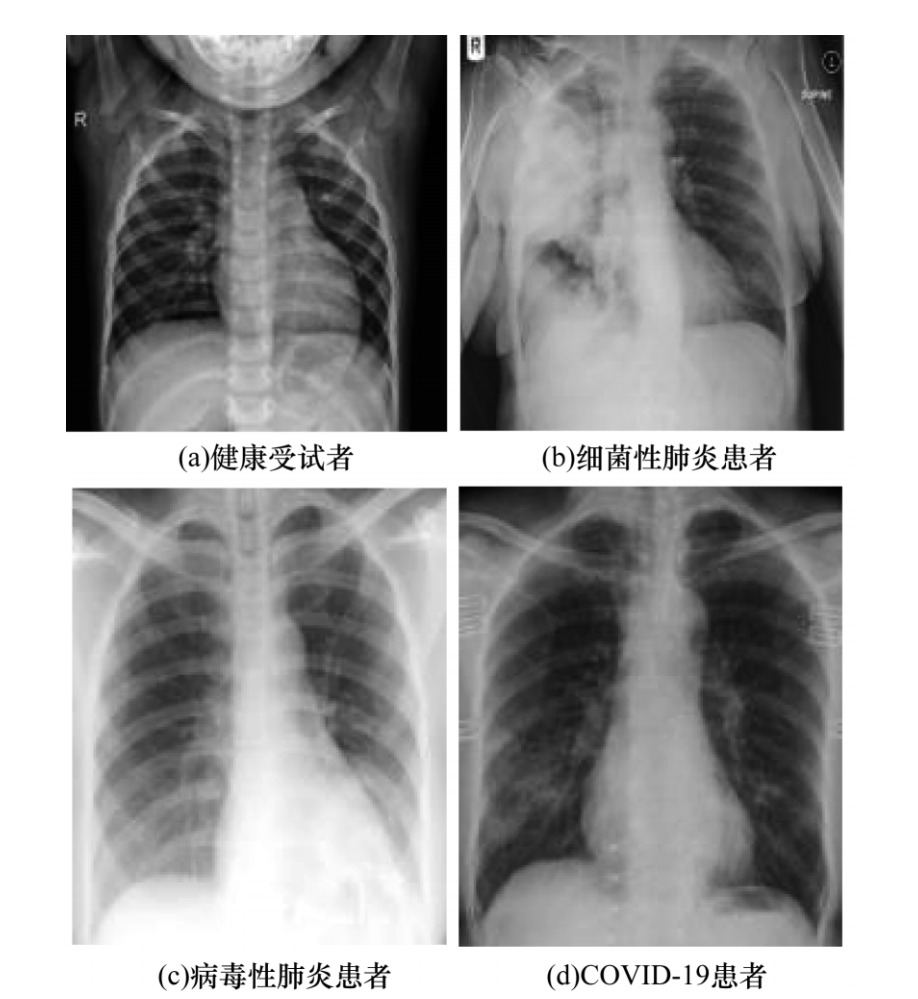
\includegraphics[width=0.4\textwidth]{img/fig15.png}
\caption{胸部X-ray样本图像}
\label{fig:figure3}
\end{figure}
\begin{figure}[h]
\centering
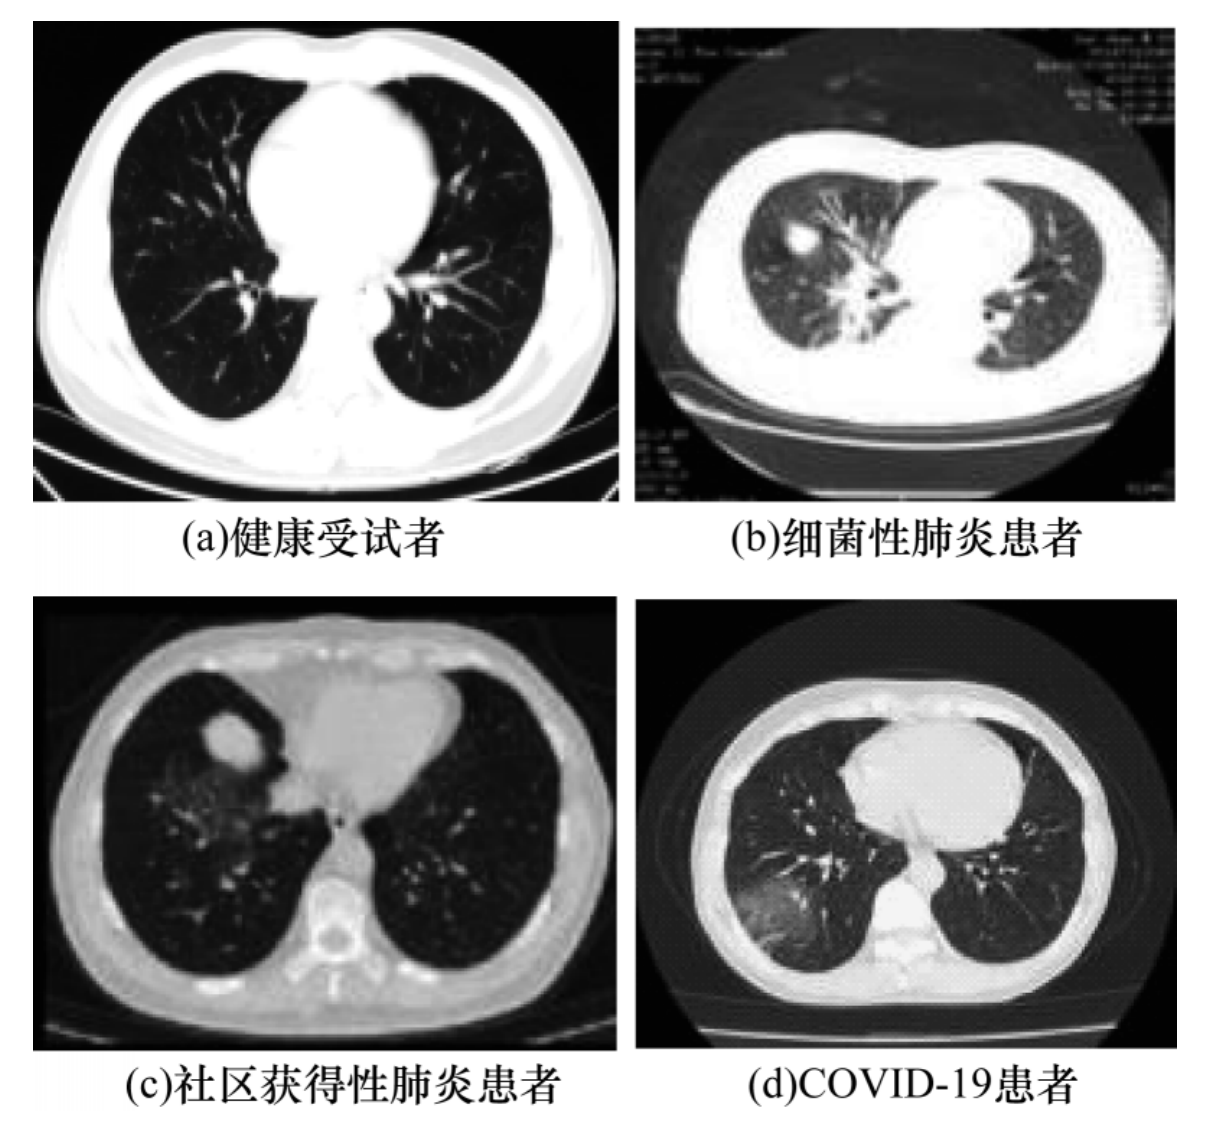
\includegraphics[width=0.4\textwidth]{img/fig16.png}
\caption{胸部CT样本图像}
\label{fig:figure3}
\end{figure}
\subsubsection{基于X-ray的COVID-19诊断模型}

文献\cite{b20}提出一种贝叶斯CNN评估COVID-19预测中的诊断不确定性。实验结果表明,在不同的MCDW(Monte-Carlo Drop Weight)下,贝叶斯推理能提高ResNet50V2模型的检测准确率,并且模型的不确定性与预测准确率之间具有强相关性。此外,该文进一步生成显著性图来说明深度网络所关注的位置,从而加深对深度学习结果的理解,做出更明智的决策。

文献\cite{b21}提出基于3种不同的深度学习模型,即基于ResNet50、Inceptionv3和Inception-ResNetv2\cite{b22}的COVID-19诊断模型,用于从X-ray图像中检测出COVID-19。通过ROC分析和5-fold交叉验证可以看出:在准确率方面,相对Inceptionv3的97.0\%和Inception-ResNetv2的87\%,ResNet50模型获得了98.0\%的最高分类性能。

文献\cite{b23}提出一个基于Efficient Net\cite{b24}的检测诊断模型,使用EfficientNet-B0网络在ImageNet上进行预训练用以提取特征,并且附带异常检测模块和置信分数预测模块。该模型包含两方面的任务:对COVID-19和非COVID-19患者进行分类,并进行异常检测。其中,异常检测任务给出异常分数,以优化用于分类的COVID-19分数。该模型的敏感性为71.7\%,特异性为73.8\%,AUC为0.836。

文献\cite{b25}提出一种基于ResNet的CNN网络模型(COVID-Net)。该模型对正常、细菌性感染、非COVID-19病毒性感染和COVID-19病毒性感染进行预测,并且满足准确率高于80\%和计算复杂度小于2.5亿次乘加运算等设计要求。COVID-Net首先在ImageNet数据集\cite{b26}上预训练,然后使用Adam优化器在COVIDx数据集上训练。COVIDx数据集包含45例COVID-19患者、1203例正常受试者、931例病毒性肺炎患者和660病毒性肺炎患者的X-ray数据。该模型的准确率为83.5\%,敏感性为100\%,精准率为80\%。

文献\cite{b27}提出利用迁移学习自动检测COVID-19。首先对近年来用于医学图像分类中最先进(SOTA)的CNN模型进行性能评估,其中包括VGG19\cite{b28}、MobleNetv2\cite{b29}、Xception\cite{b30}、Inception和Inception-ResNetv2。然后通过迁移学习\cite{b31}在小型医学图像数据集中检测异常,从而实现对COVID-19的诊断。通过对比不同的CNN结果发现,VGG19和MobileNetv2表现最佳。此外,通过计算分析最佳模型对应混淆矩阵可以看出,VGG19具有更高的准确率,其准确率为97.83\%,而MobileNetv2在敏感性方面(99.1\%)优于VGG19,因此其被证明是特定分类任务和特定数据样本的有效模型。

以上研究涉及的数据集大多来自两个数据集:COVID-chestxray-dataset,包括70张COVID-19患者肺部X-ray图像;KAG数据集,包括健康受试者、病毒性肺炎患者和细菌性患者的5863张X-ray图像。由于COVID-19图像数量有限,不足以评估以上方法的鲁棒性,导致其临床中心应用的可推广性也难以被认可。此外,X-ray作为最常用的医学成像方式之一,被广泛用于为放射科医生提供证据,但通常被认为不如胸部CT图像敏感。值得注意的是,最近一项研究报告表明\cite{b32},COVID-19患者在早期或者轻度症状阶段,X-ray显示正常。因此,研究人员尝试利用CT数据进行COVID-19的诊断。
\subsubsection{基于CT的COVID-19诊断模型}

文献\cite{b33}提出了一种弱监督检测诊断模型,利用三维CT图像检测COVID-19。首先,对于每个患者使用预训练模型U-Net分割肺部区域。然后,将分割的3D肺部区域作为三维CNN的输入,以预测感染COVID-19的概率。三维CNN包括以下3个部分:第一部分为主干网络,由1个三维卷积核、1个BN(Batch Normalization)层和1个池化层组成;第二部分由2个残差块构成;第三部分为渐进式分类器,包含3个卷积层和1个全连接层。在该工作中,收集的542名受试者(313例COVID-19、229例非COVID-19)的胸部CT图像被用作训练和测试数据。该模型的敏感性为90.7\%,特异性为91.1\%,AUC为0.959。

文献\cite{b34}提出一个用于COVID-19分类和预后分析的全自动深度学习模型。该模型使用DenseNet121\cite{b35}作为骨干网络,首先将DenseNet121与FPN相结合完成肺部区域的自动分割,然后利用类DenseNet结构(COVID-19Net)建立分类网络,对分割得到的区域进行分类。该文共收集了7个省市的5372例CT图像,包括COVID-19数据集和表皮生长因子受体(Epidermal Growth Factor Receptor,EGFR)数据集。其中,4106例具有EGFR基因突变状态的患者样本用来对模型进行预训练\cite{b36},使其学习肺部特征,924例COVID-19患者和342例其他肺炎患者样本则用来进行模型训练和验证。在4个外部验证集中,该模型从其他肺炎(AUC=0.87和0.88)和病毒性肺炎(AUC=0.86)中识别COVID-19取得了良好的效果。

文献\cite{b37}采用胸部CT扫描数据集,包含2685例样本(1658例COVID-19、1027例普通肺炎)。该模型首先对所有图像进行预处理,采用VBNet\cite{b38}分割感染区域、左/右肺、5个肺叶和18个肺段。然后提取感染大小、位置特征和放射特征等手工特征,并使用最小绝对收缩和选择算子\cite{b39}进行特征选择。在此基础上,提出一种感染区域大小感知的随机森林方法,将受试者自动分为不同感染病灶大小的分组,并在每组中进行随机森林分类。实验结果表明,该方法对于感染大小在0.01\% $ \sim $ 10\%中等范围内的病例取得了较大的性能裕度,而对小范围感染的患者被识别的敏感性较低。在5-fold交叉验证下,该模型敏感性为90.7\%,特异性为83.3\%,准确率为87.9\%。

文献\cite{b40}通过神经结构搜索(NAS)设计一个轻量级的三维模型,结合CT图像检测进行COVID-19诊断。该模型首先建立搜索空间,定义神经结构的设计原则。然后选择搜索策略,相关研究表明,随机搜索比其他许多方法更具竞争力\cite{b41}。最后选择准确率方面排名靠前的模型进行对比。作者将通过NAS搜索得到的最佳模型命名为MNas3DNet。实验结果表明,相对基线3D模型,MNas3DNet模型尺寸更小。此外,其中MNas3DNet41能实现SOTA级别的性能表现,相应的准确率为87.14\%,F1评分为87.25\%,AUC为0.957。

文献\cite{b42}提出一种基于混合密度网络模型的深度双向长短时记忆网络(DBM),并结合自适应差分进化(MADE)算法\cite{b43}构建MADE-DBM模型。该模型可以有效避免手工调整超参数的繁琐过程,适用于COVID-19实时分类系统。该文采用SARS-CoV-2CT-scan数据集,将训练集和测试集按3∶2的比例进行划分,并对提出的模型与其他SOTA模型分别进行二分类和三分类的性能比较。实验结果表明,该模型在AUC、敏感性、特异性和准确率等指标上相较于其他模型均获得了最佳表现。对于二分类,其AUC达到0.983,敏感性达到0.989,准确率达到98.4\%。

文献\cite{b44}介绍公开数据集COVID-CT-set,并且提出一种快速、准确的全自动系统用于从CT图像中检测出COVID-19患者的图像。该系统主要流程如下:在第一阶段运行优化的图像处理算法,以丢弃肺部内部无法正常显示的CT图像。在下一阶段提出一种基于ResNet50V2改进的深度卷积网络,并通过特征金字塔网络进行增强,对所选CT图像进行分类。最后利用特征可视化算法对分类后的图像进行处理,以显示图像中的感染区域。实验结果表明,该系统能够以专业医生5倍的识别速度,达到98.49\%的准确率。



\section{模型性能对比及分析}
上文对数据集、评价指标和基于深度学习技术的 COVID-19 检测诊断模型进行了详细介绍。下文将从骨干网络、数据集、数据类型、性能表现、分类种类和开源情况 6 个维度,分析比较现有基于深度学习的 COVID-19 检测诊断模型,具体见下表:
%插入图片
\begin{figure}[h]
\centering
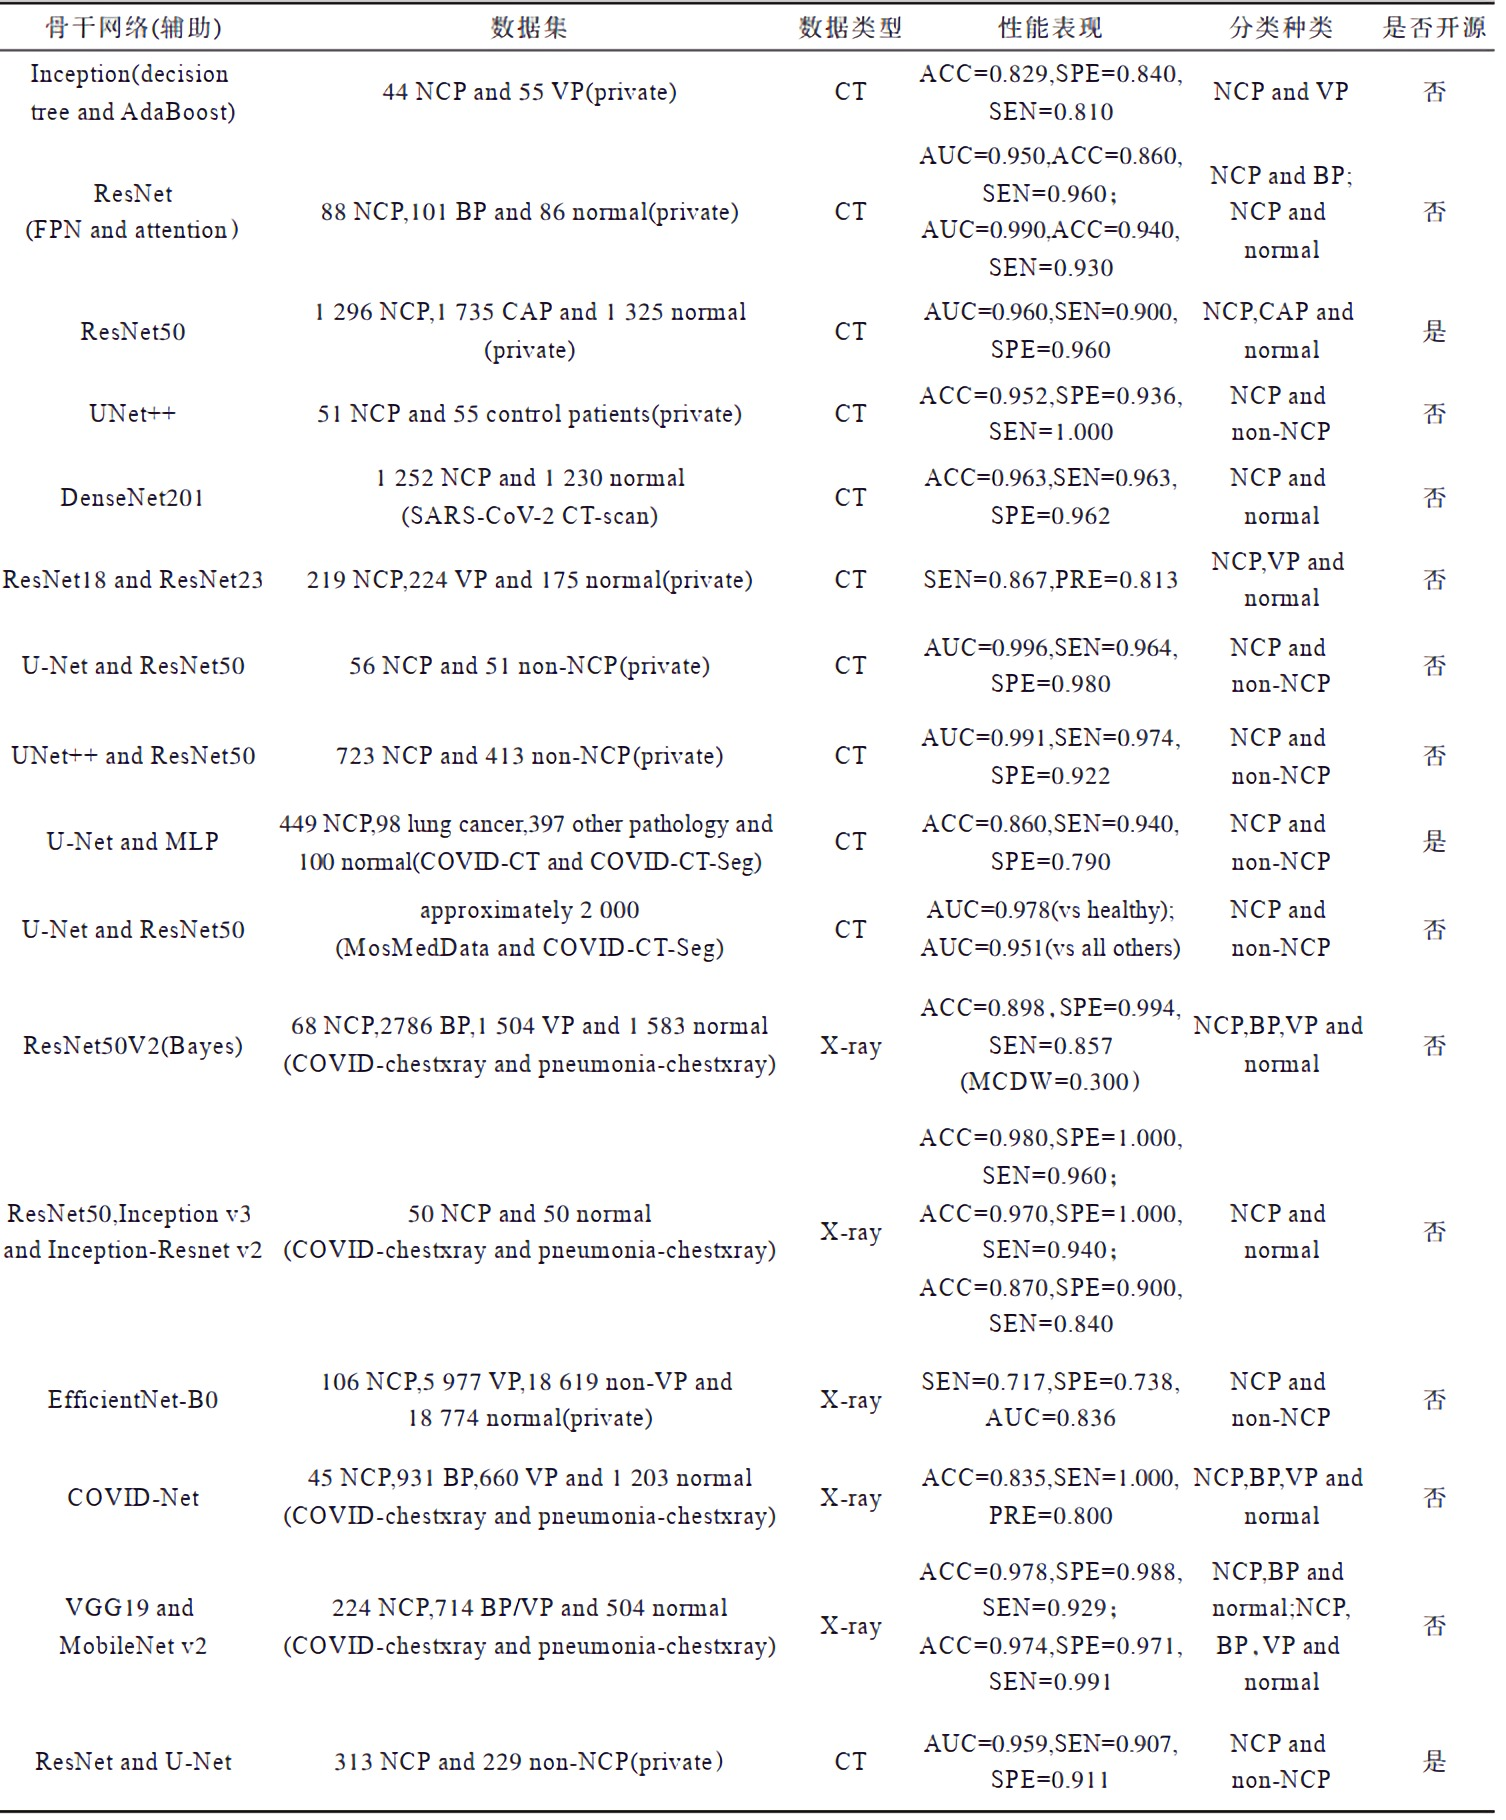
\includegraphics[width=0.5\textwidth]{img/fig1.jpg}
\caption{基于深度学习的 COVID-19 检测诊断模型性能表}
\label{fig:COVID-19_classification_and_segmentation_performance}
\end{figure}


从表中可以得出结论:
%有序列表
\begin{enumerate}
\item 对骨干网络进行分析可知:COVID-19 检测诊断模型的网络结构包含分割网络(U-Net、UNet++和VBNet 等)和分类网络(ResNet 系列、DenseNet 系列、Inception 系列等),由于 COVID-19 患者在不同阶段表现出不同的影像学特征,因此可以使用分割网络。

对 ROI 区域进行分割提取;同时可以借助分类网络学习 COVID-19 患者特有的影像学特征,从而有效区分 COVID-19、其他肺炎和正常受试者;此外,研究者 借 助 辅 助 手 段(如 FPN、注 意 力 机 制 、决 策 树 、Lasso 等)可有效提高模型的性能。
\item 对 数 据 集 进 行 分 析 可 知 :多 数 研 究 工 作 的COVID-19 数据集样本数量范围从几十到几百不等,大部分研究者采用迁移学习,并基于小样本COVID-19数据集进行检测诊断;此外,目前只有极少量公开可用的大型 COVID-19影像数据集(如 CC-CCII数据集、MosMedData 数据集、SARS-CoV-2CT-scan 数据集、COVID-CT-set数据集),大部分研究人员采用私有数据集,由此也导致部分模型的泛化能力较弱,对特定数据集有一定的偏移性,因此,无法在相对公平的条件下通过比 较 不 同 数 据 集 下 的 实 验 结 果 来 评 价 模 型 性 能优劣。
\item 对影像类型进行分析可知:科研工作者倾向基于 CT 图像的 COVID-19 诊断,一方面,因为 X-ray 相对 CT 图像敏感性更低;另一方面,CT 图像数据除了二维类型外,还包含更多深层次三维特征信息 ,CNN 在图像处理方面的出色表现,本质上源于其强大的特征提取能力,因此,CNN能够从三维 CT 图像数据中获取更多的特征信息,从而提高诊断的效果。
\item 对分类种类分析可知:上述模型的 COVID-19分类任务可归纳为二分类(COVID-19与non COVID-19)、三分类(COVID-19、其他肺炎和正常)以及四分类(COVID-19、其他病毒性肺炎、细菌性肺炎和正常)。
\item 对开源情况进行分析可知:只有少量模型开源。由于各个模型之间进行直接比较缺乏一定的公正性,后续可以通过统一的数据集建立相对公平的环境,对目前现有的开源模型进行比较实验,因此对数据集的统一完善以及开源模型的改进显得至关重要。综上,现有基于深度学习的 COVID-19 诊断模型从不同角度进行新冠肺炎的检测诊断,并取得了不错的表现。这些模型不仅能够完成对 ROI 区域的自动分割和自动标注,有效减少医务人员的人工操作,而且还能对 COVID-19 患者进行快速筛选,辅助专业人士进行高效诊断。
\end{enumerate}
\section{应用实例介绍}
目前,多种基于深度学习的COVID-19检测诊断模型相继被提出,并经过不断的优化完善,性能已可满足实际应用场景下的临床应用需求。特别是利用CT图像辅助诊断COVID-19的肺炎AI影像辅助产品,极大提高了临床诊断效率,在COVID-19的防控工作中发挥了举足轻重的作用。下文将介绍在抗疫场景下表现出色的人工智能应用系统。


阿里达摩院医疗AI团队基于最新的诊疗方案,包括钟南山院士等多个权威团队发表的关于新冠肺炎患者临床特征的工作,与浙大一附院、万里云、长远佳和古珀医院等多家机构开展合作,率先突破了训练数据不足的局限,其基于5000多个病例的CT影像样本数据学习、训练样本的病灶纹理,研发了全新的AI算法模型。该技术能够在20s内对患者的肺部CT图像作出分析和判读,从而为临床医生的诊断提供有力依据,准确率达到96\%以上。此外,该技术还可计算病灶部位的比例,量化、预测病症的轻重程度,大幅度提升诊断效率,为患者的治疗争取宝贵时间。特别是对未接诊过新冠肺炎病例或低年资医生,可提供有效的诊断鉴别提示信息。同时,阿里达摩院还与阿里云共同研发了辅助诊断算法,该算法可以根据患者的基本信息、症状、实验室检查结果、流行病学史、影像报告等多维信息,进一步辅助医生制定科学的治疗方案。


依图胸部CT的COVID-19智能评价系统由上海市公共卫生临床中心和依图医疗合作开发,其作为业界首个COVID-19智能影像评价系统于2020年1月28日上线。该系统可实现前中后期的全流程辅助诊断,并采用创新的AI全肺定量分析技术,提升诊断的速度和精度,帮助医生进行快速检出、定量检测和疗效评价。该系统具体功能和性能为:

%有序列表
\begin{enumerate}
\item 智能检出:肺炎病变检出率敏感性达97.3\%,特异性达99\%。
\item 智能分析:对肺炎严重程度进行量化评价,在2s $ \sim $ 3s内完成定量分析。
\item 智能随访:智能随访分析患者病程,精准匹配历史影像,自动分析病情的转移和发展。
\end{enumerate}

钟南山等专家通过召集支援武汉一线工作富有临床经验的医师,并联合统计学、生物医学工程和信息技术领域的专家,开发了基于物联网医学技术的COVID-19智能诊治辅助程序,简称nCapp。该程序主要包括以下3个方面的功能:
\begin{enumerate}
\item 智能辅助诊断:根据提供的数据、问卷回复以及检查结果自动进行确诊,并对疑似和可疑的病例进行归类;根据患者病情的严重程度,区分为轻型、普通型、重型和危重型;建立实时更新的COVID-19样例数据库,通过最新病例数据对智能诊断的算法模型进行实时优化升级,提升诊断的准确率。
\item 智能指导治疗:对不同类型患者制定不同的治疗方案,追踪COVID-19愈后患者情况,进行长期随访管理。
\item 智能数据监测:自主监控上传至云服务器数据的可靠性与真实性,保证nCapp能够有效地辅助专家进行诊断。
\end{enumerate}

张康教授团队研发的COVID-19智慧筛查、诊断与预测系统,可以对大量疑似肺炎病人进行快速筛查、辅助诊断和住院临床分级预警,实现对COVID-19病人的全生命周期管理。该团队基于五十万份临床影像学大数据,运用深度学习、迁移学习和语义分割等多种AI前沿技术,开发基于胸部CT和X-ray的新冠肺炎AI辅助诊断系统。该系统可在20s内完成检测及诊断过程,且诊断准确率达90\%以上。此外,其还具有病情严重程度分级和重症危重症预测功能,可对胸部CT图像每一层面的小结节、磨玻璃影和实变进行自动识别、标注及定量分析,通过患者的吸氧频率、血氧饱和度、酸碱平衡、肝功能、凝血功能等信息,综合预测病人发展为重症、危重症的概率和时间,有利医生进行及时干预,降低患者死亡率。
\section{未来研究方向}
现有多数基于深度学习的 COVID-19 检测诊断模型都是基于小样本数据集训练得到的,这可能会导致结果的过拟合,且不足以产生稳健的预测。因此,为提高模型性能,使其能够更好地辅助临床诊断,COVID-19 数据集的质量和数量都有待进一步提高。在数量方面,需要联合多家医院和研究机构,实现资源共享以扩大样本量;在质量方面,要求所有的影像数据都是规范的和标准的,并需要对这些影像数据进行精确标记。在训练方法上,我们利用迁移学习技术来研究。从头开始训练一个深度 CNN 需要很长时间,而训练后的 CNN 的表现可能远不能令人满意。在迁移学习中,把在不同数据集上训练好的网络作为基础网络,利用待研究的数据集可以训练调整后的网络。迁移学习可以缩短训练时间,同时可以在小样本数据集上取得较好的训练效果。

值得注意的是,影像数据中不完整、不精确的标记,将显著降低诊断模型性能,而基于弱监督深度学习技术的COVID-19 诊断模型可以有效规避噪声数据(或低质量数据)的影响,这将是未来诊断模型一个较好的发展方向。此外,数据的人工标注往往费时费力,研究者可以尝试利用无监督和自监督等方法构建COVID-19 诊断模型。

由于新冠影像质量受到不同地区、人种、病毒类型、摄像设备型号的影响,最终实际进行测试的新冠图像与训练数据可能存在质量差异,导致模型的泛化能力并不理想。因此在实际应用中,针对不同噪声攻击做出防御,提升模型面对各种对抗扰动的鲁棒性具有重要意义。研究中可采取对抗训练算法,在训练过程中引入微小扰动以提升模型鲁棒性。

虽然深度学习在医疗图像的分析上取得了巨大成功, 然而深度学习是一个复杂的非线性系统,从输入到输出的具体决策过程不够透明,可解释性弱。但是,一个医疗诊断系统必须是透明的、可理解的、可解释的,才能获得医生、监管者和病人的信任。因此,可视化训练过程以提升模型可解释性也是一项重要工作。

此外,传统深度学习模型通常由一个复杂的结构组成,在训练和使用时需要占用大量内存和 GPU资源。对于中小型医院和患者来说成本过高、难以部署,且无法接入嵌入式设备。
进行模型压缩有利于Al辅助诊断系统在医疗资源匮乏地区的推广和落地。

与此同时,新冠肺炎诊断不应仅局限于COVID-19 和普通肺炎之间的分类,而应扩展至细粒度或者精细化研究,由此分析得出患者的感染患病等级。另外,还应聚焦于对病情发展情况的预测,以便及时转移、治疗有明显恶化趋势的病人,更合理地分配医疗资源。

当下一些热门的深度学习方法同样值得借鉴,如多组学分析、多任务学习分析、图卷积神经网络和vision transformer(ViT)等。
\section{结语}
在新冠肺炎的诊断和治疗中,深度学习的技术被广泛应用。AI技术不仅降低了抗击疫情的人力、物理成本,同时为医疗资源贫乏地区的疫情防控提供了帮助。本文结合基于深度学习的新冠肺炎诊断模型研究现状,总结了新冠数据集的相关情况,并将目前性能较为突出的医学图像特征提取、分割和分类方法进行整理和评估,并总结了模型的评估方法。本文还对相关文献的典型模型进行了分析概括。随着相关检测诊断模型研究不断发展,效果显著的模型被陆续提出并被成功应用到抗击新冠肺炎的第一线,这对扼制新冠肺炎大规模流行具有重大意义。尽管AI辅助新冠诊断已经取得了许多突出的成就,但研究中仍有众多挑战和难题。因此,本文还针对AI辅助新冠肺炎领域存在的问题,总结提出了其未来发展方向,以推动该领域的发展。

%\section{参考文献}
\begin{thebibliography}{00}
    \bibitem{b1} Wang S ,  Kang B ,  Ma J , et al. A deep learning algorithm using CT images to screen for Corona virus disease (COVID-19)[J]. European Radiology, 2021(1).

    \bibitem{b2} Szegedy C ,  Wei L ,  Jia Y , et al. Going deeper with convolutions[C]// 2015 IEEE Conference on Computer Vision and Pattern Recognition (CVPR). IEEE, 2015.
    
    \bibitem{b3} Hui Z ,  Zhu J ,  Rosset S , et al. Multi-class AdaBoost.  2009.
    
    \bibitem{b4} Song Y ,  Zheng S ,  Li L , et al. Deep learning Enables Accurate Diagnosis of Novel Coronavirus (COVID-19) with CT images[J]. IEEE/ACM Transactions on Computational Biology and Bioinformatics, 2021, PP(99):1-1.
    
    \bibitem{b5} He K ,  Zhang X ,  Ren S , et al. Deep Residual Learning for Image Recognition[J]. IEEE, 2016.
    
    \bibitem{b6} Lin T Y ,  Dollar P ,  Girshick R , et al. Feature Pyramid Networks for Object Detection[C]// 2017 IEEE Conference on Computer Vision and Pattern Recognition (CVPR). IEEE Computer Society, 2017.
    
    \bibitem{b7} Fu J ,  Zheng H ,  Tao M . Look Closer to See Better: Recurrent Attention Convolutional Neural Network for Fine-Grained Image Recognition[C]// IEEE Conference on Computer Vision \& Pattern Recognition. IEEE, 2017.
    
    \bibitem{b8} Li L ,  Qin L ,  Xu Z , et al. Artificial Intelligence Distinguishes COVID-19 from Community Acquired Pneumonia on Chest CT.  2020.
    
    \bibitem{b9} Chen J ,  Wu L ,  Zhang J , et al. Deep learning-based model for detecting 2019 novel coronavirus pneumonia on high-resolution computed tomography[J]. Scientific Reports.
    
    \bibitem{b10} Zhou Z ,  Siddiquee M ,  Tajbakhsh N , et al. UNet++: A Nested U-Net Architecture for Medical Image Segmentation[C]// 4th Deep Learning in Medical Image Analysis (DLMIA) Workshop. 2018.
    
    \bibitem{b11} Ronneberger O ,  Fischer P ,  Brox T . U-Net: Convolutional Networks for Biomedical Image Segmentation[C]// International Conference on Medical Image Computing and Computer-Assisted Intervention. Springer International Publishing, 2015.
    
    \bibitem{b12} Kumar V ,  Jaiswal A ,  Gianchandani N , et al. Classification of the COVID-19 infected patients using DenseNet201 based deep transfer learning[J]. Journal of biomolecular Structure \& Dynamics, 2020(1).
    
    \bibitem{b13} Xu X ,  Jiang X ,  Ma C , et al. Deep Learning System to Screen Coronavirus Disease 2019 Pneumonia[J]. arXiv, 2020.
    
    \bibitem{b14} Hara K ,  Kataoka H ,  Satoh Y . Learning Spatio-Temporal Features with 3D Residual Networks for Action Recognition[J]. arXiv e-prints, 2017.
    
    \bibitem{b15} Gozes O ,  Frid-Adar M ,  Greenspan H , et al. Rapid AI Development Cycle for the Coronavirus (COVID-19) Pandemic: Initial Results for Automated Detection \& Patient Monitoring using Deep Learning CT Image Analysis[J]. arXiv e-prints, 2020.
    
    \bibitem{b16} He K ,  Zhang X ,  Ren S , et al. Identity Mappings in Deep Residual Networks[C]// European Conference on Computer Vision. Springer International Publishing, 2016.
    
    \bibitem{b17} Wang B ,  Jin S ,  Yan Q , et al. AI-assisted CT imaging analysis for COVID-19 screening: Building and deploying a medical AI system[J]. Applied Soft Computing, 2020:106897.
    
    \bibitem{b18} Amyar A ,  Modzelewski R ,  Hua L , et al. Multi-task deep learning based CT imaging analysis for COVID-19 pneumonia: Classification and segmentation[J]. Computers in Biology and Medicine, 2020, 126:104037.
    
    \bibitem{b19}Rich, Caruana. Multitask Learning[J]. Machine Learning, 1997.
    
    \bibitem{b20} Goncharov M ,  Pisov M ,  Shevtsov A , et al. CT-based COVID-19 Triage: Deep Multitask Learning Improves Joint Identification and Severity Quantification[J]. Medical Image Analysis, 2021(1):102054.
    
    \bibitem{b21} Ghoshal B ,  Tucker A . Estimating Uncertainty and Interpretability in Deep Learning for Coronavirus (COVID-19) Detection[J].  2020.
    
    \bibitem{b22} Narin A ,  Kaya C ,  Pamuk Z . Automatic Detection of Coronavirus Disease (COVID-19) Using X-ray Images and Deep Convolutional Neural Networks[J].  2020.
    
    \bibitem{b23} Szegedy C ,  Ioffe S ,  Vanhoucke V , et al. Inception-v4, Inception-ResNet and the Impact of Residual Connections on Learning[J].  2016.
    
    \bibitem{b24} Zhang J ,  Xie Y ,  Liao Z , et al. Viral Pneumonia Screening on Chest X-ray Images Using Confidence-Aware Anomaly Detection[J]. arXiv e-prints, 2020.
    
    \bibitem{b25} Tan M ,  Le Q V . EfficientNet: Rethinking Model Scaling for Convolutional Neural Networks[J].  2019.
    
    \bibitem{b26} Wang L ,  Lin Z Q ,  Wong A . COVID-Net: a tailored deep convolutional neural network design for detection of COVID-19 cases from chest X-ray images[J]. Scientific Reports, 2020, 10(1).
    
    \bibitem{b27} Jia D ,  Wei D ,  Socher R , et al. ImageNet: A large-scale hierarchical image database[C]// 2009:248-255.
    
    \bibitem{b28} Apostolopoulos I D ,  Bessiana T . Covid-19: Automatic detection from X-Ray images utilizing Transfer Learning with Convolutional Neural Networks[J].  2020.
    
    \bibitem{b29} Simonyan K ,  Zisserman A . Very Deep Convolutional Networks for Large-Scale Image Recognition[J]. Computer Science, 2014.
    
    \bibitem{b30} Howard A G ,  Zhu M ,  Chen B , et al. MobileNets: Efficient Convolutional Neural Networks for Mobile Vision Applications[J].  2017.
    
    \bibitem{b31} Chollet F . Xception: Deep Learning with Depthwise Separable Convolutions[C]// 2017 IEEE Conference on Computer Vision and Pattern Recognition (CVPR). IEEE, 2017.
    
    \bibitem{b32}Pan, S. J.,Tsang, I. W.,Kwok, J. T.,Yang, Q. Domain Adaptation via Transfer Component Analysis[J]. IEEE Transactions on Neural Networks, 2011, 22(2):199-210.
    
    \bibitem{b33} Zheng C ,  Deng X ,  Fu Q , et al. Deep Learning-based Detection for COVID-19 from Chest CT using Weak Label.  2020.
    
    \bibitem{b34} Wang S ,  Zha Y ,  Li W , et al. A Fully Automatic Deep Learning System for COVID-19 Diagnostic and Prognostic Analysis.  2020.
    
    \bibitem{b35} Huang G ,  Liu Z ,  Laurens V , et al. Densely Connected Convolutional Networks[C]// IEEE Computer Society. IEEE Computer Society, 2016.
    
    \bibitem{b36}Shuo, Wang, Jingyun, et al. Predicting EGFR mutation status in lung adenocarcinoma on computed tomography image using deep learning.[J]. European Respiratory Journal, 2019.
    
    \bibitem{b37} Shi F ,  Xia L ,  Shan F , et al. Large-Scale Screening of COVID-19 from Community Acquired Pneumonia using Infection Size-Aware Classification[J]. arXiv, 2020.
    
    \bibitem{b38} Shan F ,  Gao Y ,  Wang J , et al. Lung Infection Quantification of COVID-19 in CT Images with Deep Learning[J]. arXiv, 2020.
    
    \bibitem{b39} He X ,  Liu J ,  Ibrahim J , et al. Journal of the American Statistical Association[J]. american statistician.
    
    \bibitem{b40} He X ,  Wang S ,  Shi S , et al. Benchmarking Deep Learning Models and Automated Model Design for COVID-19 Detection with Chest CT Scans.  2020.
    
    \bibitem{b41} Liam L I ,  University C M ,  Determined A I . Random Search and Reproducibility for Neural Architecture Search.
    
    \bibitem{b42} Pham H ,  Guan M Y ,  Zoph B , et al. Efficient Neural Architecture Search via Parameter Sharing[J].  2018.
    
    \bibitem{b43} Yu K ,  Sciuto C ,  Jaggi M , et al. Evaluating the Search Phase of Neural Architecture Search[J].  2019.
    
    \bibitem{b44} Pathak Y ,  Shukla P K ,  Arya K V . Deep bidirectional classification model for COVID-19 disease infected patients[J]. IEEE/ACM Transactions on Computational Biology and Bioinformatics, PP(99):1-1.
    
\end{thebibliography}
\end{document}
